% 번역본 공통 서식. tectonic으로 컴파일.
\documentclass[11pt,a4paper]{article}
\usepackage{fontspec}
\usepackage{xeCJK}
\setCJKmainfont[BoldFont={Apple SD Gothic Neo Bold},ItalicFont={AppleMyungjo},ItalicFeatures={FakeSlant=0.18}]{AppleMyungjo}
\setCJKsansfont{Apple SD Gothic Neo}
\setCJKmonofont{Apple SD Gothic Neo}
\xeCJKsetup{CJKspace=true,CJKecglue={},xCJKecglue=false}
\usepackage{amsmath,amssymb,mathtools,bm}
\usepackage[margin=24mm]{geometry}
\usepackage{booktabs,tabularx,array,multirow}
\usepackage{graphicx}
\usepackage{enumitem}
\usepackage{xcolor}
\usepackage[hidelinks]{hyperref}
\linespread{1.3}
\setlength{\parskip}{0.35em}
\newcolumntype{Y}{>{\raggedright\arraybackslash}X}
\newcommand{\E}{\mathbb{E}}
\newcommand{\Var}{\operatorname{Var}}
\renewcommand{\P}{\mathbb{P}}
\newcommand{\Q}{\mathbb{Q}}
\newcommand{\dd}{\mathsf{d}}   % 왜곡 척도 d (원문 산세리프)
\newcommand{\ff}{\mathsf{f}}
\renewcommand{\gg}{\mathsf{g}}  % 주의: ≫ 는 \ggg 대신 \gg 사용 불가
\newcommand{\ttl}{\jmath}      % d-기울인 정보 ȷ
\newcommand{\iinf}{\imath}     % 정보 확률변수 ı
\newcommand{\onote}[1]{\footnote{[옮긴이] #1}}
\renewcommand{\figurename}{그림}
\renewcommand{\tablename}{표}
\renewcommand{\abstractname}{초록}

\usepackage{fancyhdr}
\pagestyle{fancy}\fancyhf{}
\fancyhead[L]{\small 유한 부호 길이 정보이론 (한국어 번역)}
\fancyhead[R]{\small arXiv:2504.07743v2}
\fancyfoot[C]{\small\thepage}
\renewcommand{\headrulewidth}{0.3pt}

\begin{document}

\noindent\fbox{\parbox{\dimexpr\linewidth-2\fboxsep-2\fboxrule}{\small
\textbf{번역본 안내.}
이 문서는 J.~Gao, S.~Chen, Y.~Wu, L.~Liu, G.~Caire, H.~V.~Poor, W.~Zhang,
``Finite-Blocklength Information Theory,'' arXiv:2504.07743v2 [cs.IT], 2025년 12월 25일
(\url{https://arxiv.org/abs/2504.07743})을 한국어로 옮긴 것이다.
원문은 크리에이티브 커먼즈 저작자표시 4.0 국제 라이선스(CC BY 4.0,
\url{https://creativecommons.org/licenses/by/4.0/})로 공개되어 있으며, 이 번역본도 같은 조건을 따른다.
\textbf{변경 사항:} 본문·캡션·각주를 한국어로 옮겼고, 표 1과 수식은 다시 조판했으며, 그림은 원문에서 잘라 실었다.
참고문헌은 원문 그대로 두었다. ``[옮긴이]''로 시작하는 각주는 원문에 없는 번역자의 주석이다.
원저자는 이 번역을 검토하거나 보증하지 않았다. 인용할 때는 원문을 인용한다.
}}
\vspace{1em}

% ===== Part A: 원문 PDF 1–10쪽 (제목, 초록, 1장, 2장 도입, 2.1, 2.2) =====
\begin{center}
{\LARGE 유한 부호 길이 정보이론\par}
\vspace{0.4em}
{\large Finite-Blocklength Information Theory\par}
\vspace{1.2em}
Junyuan Gao\textsuperscript{a,b}, Shuao Chen\textsuperscript{b}, Yongpeng Wu\textsuperscript{b,$*$}, Liang Liu\textsuperscript{a}, Giuseppe Caire\textsuperscript{c}, H. Vincent Poor\textsuperscript{d}, Wenjun Zhang\textsuperscript{b}\par
\vspace{0.8em}
{\small\itshape
\textsuperscript{a}Department of Electrical and Electronic Engineering, The Hong Kong Polytechnic University, Hong Kong SAR, China\par
\textsuperscript{b}Department of Electronic Engineering, Shanghai Jiao Tong University, Shanghai, Minhang 200240, China\par
\textsuperscript{c}Communications and Information Theory Group, Technische Universität Berlin, Berlin, 10587, Germany\par
\textsuperscript{d}Department of Electrical and Computer Engineering, Princeton University, Princeton, NJ 08544, USA\par}
\vspace{0.6em}
{\small \textsuperscript{$*$}교신저자. 이메일: \texttt{yongpeng.wu@sjtu.edu.cn} (Yongpeng Wu)\par}
\end{center}

\begin{quote}
\textbf{초록}\par
무선 통신 시스템의 근본 한계(fundamental limit)를 다루는 전통적인 점근(asymptotic) 정보이론 연구는 주로 몇 가지 이상적인 가정에 기대어 왔다. 부호 길이(blocklength)가 무한하고 오류 확률이 0으로 사라진다는 가정이 대표적이다. 이러한 가정 덕분에 수학적으로 다루기 쉬운(tractable) 결과를 얻을 수 있지만, 새로 등장하는 차세대 무선 응용의 엄격한 요구 조건은 담아내지 못한다. 초고신뢰 저지연 통신(ultra-reliable low latency communication)이나 초대규모 기계형 통신(ultra-massive machine type communication) 같은 응용은 짧은 패킷 통신(short-packet communication), 극히 낮은 지연, 낮은 에너지 소비 등 훨씬 폭넓은 특성을 지원해야 한다. 이런 응용을 더 잘 뒷받침하려면 유한 부호 길이(finite blocklength) 정보이론을 고려해야 한다. 이 논문은 이 분야의 진전을 포괄적으로 살펴본 뒤 미해결 문제를 논의한다. 구체적으로, 먼저 비점근(non-asymptotic) 영역에서 원천 부호화(source coding)의 근본 한계를 다룬다. 이때 점대점(P2P, point-to-point) 및 다중 단말(multiterminal) 환경의 무손실 압축(lossless compression)과 손실 압축(lossy compression)에 특히 초점을 맞춘다. 이어서 P2P 채널, 다중 접속 채널(multiple access channel), 새로 떠오르는 대규모 접속 채널에서 채널 부호화(channel coding)의 근본 한계를 논의한다. 나아가 결합 원천-채널 부호화(joint source and channel coding)의 최근 진전을 소개하고, 비점근 영역에서 이 방식이 분리 원천-채널 부호화(separate source and channel coding)보다 성능 면에서 상당히 앞선다는 점을 부각한다. 각 부분에서는 다양한 비점근 달성 가능성 한계(achievability bound), 역 한계(converse bound), 근사(approximation)와 그 밑바탕의 핵심 아이디어를 검토한다. 이러한 한계와 근사는 미래 무선 통신 시스템 설계에 공학적 통찰(insight)을 주는 데 꼭 필요하다.

\medskip
\textit{주제어:} 근사, 유한 부호 길이 정보이론, 저지연, 비점근 한계, 원천 및 채널 부호화
\end{quote}

\section{서론}

초고신뢰 저지연 통신(URLLC, ultra-reliable low latency communications)은 5세대(5G) 무선 네트워크의 3대 주요 사용 사례 가운데 하나이다. URLLC는 종단 간 지연과 신뢰도에 대한 요구가 엄격한 핵심 응용의 토대가 된다 [1]. 산업 자동화, 자율 주행, 원격 의료, 증강 현실(AR, augmented reality), 가상 현실(VR, virtual reality) 등이 그 예이다. 이런 응용을 지원하기 위해 3세대 파트너십 프로젝트(3GPP, 3rd generation partnership project)는 5G 네트워크에 대한 전형적인 URLLC 요구 조건으로 물리 계층 지연 1~ms와 신뢰도 99.999\%를 규정했다 [2, 3]. 다가올 6세대(6G) 무선 네트워크에서는 지연이 밀리초에서 밀리초 미만, 나아가 마이크로초 수준까지 줄고, 신뢰도는 99.999\%에서 99.9999\%로 높아질 것으로 예상된다 [4, 5]. URLLC는 더 폭넓은 신규 응용을 지원하는 데 핵심 역할을 할 것이다. 여기에는 5G 응용의 추가 발전뿐 아니라 실시간 인간-기계 상호작용, 완전 자율 주행, 인간 중심 몰입형 통신 같은 새로운 시나리오도 포함된다 [6, 7]. URLLC를 달성하는 열쇠는 더 짧은 부호 길이에서 더 신뢰성 있게 통신하는 데 있다.

Shannon의 점근 정보이론 결과는 몇 가지 이상적인 가정에 주로 기대어 무선 통신 시스템의 근본 한계를 규명한다. 무한한 부호 길이, 무한한 페이로드 크기(payload size), 0으로 사라지는 오류 확률이 그런 가정이다 [8]. 이 가정 덕분에 원천 부호화에서 달성 가능한 최소 부호율(coding rate)과 채널 부호화에서 달성 가능한 최대 부호율을 수학적으로 다루기 쉽게 규명할 수 있다. 그러나 앞서 언급한 여러 신규 응용의 엄격한 요구 조건은 이 가정으로 담아낼 수 없다. 이런 응용은 짧은 패킷 통신, 극히 낮은 지연, 작지만 무시할 수 없는 오류 확률 등 훨씬 폭넓은 특성을 지원해야 하기 때문이다. 이상적인 가정과 실제 시스템의 특성이 어긋나면서, 실제 통신 시스템의 근본 한계를 규명하는 데 점근 정보이론이 지닌 한계가 드러난다. 따라서 엄밀한 비점근 틀을 탐구하는 일이 꼭 필요하다. 이 작업에는 유한 부호 길이 영역의 난제를 풀어 갈 새로운 분석 도구와 기법이 요구된다.

\begin{figure}[t]
\centering
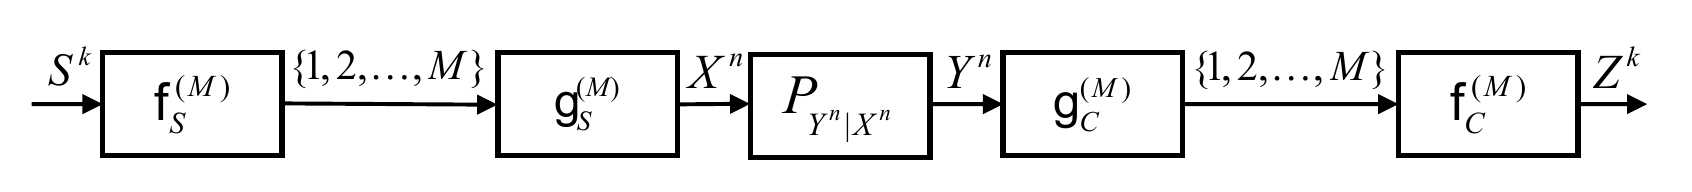
\includegraphics[width=0.85\linewidth]{fig/fig1.png}
\caption{원천 부호화와 채널 부호화의 구성.}
\end{figure}

최근 몇 년 사이 유한 부호 길이 정보이론은 원천 부호화, 채널 부호화, 결합 원천-채널 부호화(JSCC, joint source-channel coding)에 걸쳐 큰 관심을 받아 왔다. 원천-채널 부호화의 구성을 그림~1에 나타냈다. 원천 부호화, 곧 데이터 압축에서는 길이 $k$인 원천 출력 수열을 집합 $\{1,\dots,M\}$의 비트열로 사상한다. 그러면 수신 측에서 원천 기호를 정확히 복원하거나(거의 무손실 압축의 경우), 일정한 왜곡 충실도 안에서 복원할 수 있다(손실 압축의 경우). 이때 원천 알파벳 $\mathcal{S}$, 복원 알파벳 $\mathcal{Z}$, 왜곡 척도(distortion measure) $\dd:\mathcal{S}\times\mathcal{Z}\mapsto[0,+\infty]$가 주어진다. 원천 부호화의 유한 부호 길이 정보이론은 부호 길이 $k$, 오류 확률, 부호율 $\log M/k$라는 세 양 사이의 상충 관계(tradeoff)에 초점을 둔다 [10]. 여기서 오류 확률은 이산 원천 $S$에 대한 (거의) 무손실의 경우 $\P[S\neq Z]$ [9]이고, 손실의 경우 $\P[\dd(S,Z)>d]$이다. 채널 부호화의 기본 과제는 잡음이 있는 채널로 $M$개의 메시지를 부호 길이 $n$으로 전송하여, 수신 측이 $\epsilon$ 미만의 오류 확률로 메시지를 구별할 수 있게 하는 것이다 [11]. 이 경우 근본 문제는 부호 길이 $n$, 오류 요구 조건 $\epsilon$, 데이터율 $\log M/n$ 사이의 상충 관계를 규명하는 데 있다. 오늘날 대부분의 통신 시스템은 앞서 말한 원천 부호화와 채널 부호화를 차례로 수행하며, 이를 분리 원천-채널 부호화(SSCC, separate source-channel coding)라 한다. 그러나 이 구조는 유한 부호 길이에서 성능 손실이 크기 때문에, 원천과 채널의 부호기와 복호기를 함께 설계할 필요가 있다. 이런 JSCC 방식에서는 원천이 만든 길이 $k$인 수열을 채널 전송에 알맞은 길이 $n$인 수열로 직접 사상하므로, 데이터율은 $k/n$이 된다. 이때 $k$, $n$, 오류 확률 사이의 근본적인 상충 관계가 매우 중요하다 [12].

유한 부호 길이 영역에서는 위에서 말한 상충 관계를 해석적으로 정확히 기술하기 어렵다. 그래서 연구자들은 다음과 같은 촘촘하고(tight) 계산 가능한 달성 가능성 한계, 역 한계, 근사를 개발하는 쪽으로 방향을 돌린다.
\begin{itemize}
\item 달성 가능성 한계: 부호책 크기(code size) $M$, 부호 길이(원천 부호화에서는 $k$, 채널 부호화에서는 $n$), 오류 확률 $\epsilon$인 부호가 존재하면, 삼중쌍 $(M, k\ \text{또는}\ n, \epsilon)$을 달성 가능하다고 한다. 더 일반적으로 JSCC에서는 원천 입력 길이 $k$, 채널 부호 길이 $n$, 오류 확률 $\epsilon$인 결합 원천-채널 부호가 존재하면 삼중쌍 $(k,n,\epsilon)$이 달성 가능하다. 달성 가능성 한계는 달성 가능 영역의 내부 한계를 제공한다. 즉 매개변수 $(M, k\ \text{또는}\ n, \epsilon)$ 또는 $(k,n,\epsilon)$의 어떤 부분집합에 대해 부호가 존재함을 보장한다.
\item 역 한계: 역 한계는 비존재 결과를 제공한다. 즉 매개변수 $(M, k\ \text{또는}\ n, \epsilon)$ 또는 $(k,n,\epsilon)$의 특정 값에 대해서는 어떤 부호도 존재하지 않음을 보인다. 역 영역이 달성 가능 영역의 여집합과 일치하면 촘촘한 결과를 얻은 것이다. 다시 말해 가능한 가장 큰 영역을 결정한 것이다.
\item 근사: 많은 경우 영역을 촘촘하게 규명하는 일은 어떤 점근 영역에서만 가능하다(전형적인 영역은 $k$ 또는 $n\to\infty$이고 $\epsilon\to 0$인 경우이다). 그러나 $M$, $k$ 또는 $n$, $\epsilon$의 모든 비점근 값에 대해, 영역의 스케일링 법칙을 지배적인 항으로(상수 차이까지) 기술할 수 있는 경우가 흔하다. 또한 대수의 법칙과 에르고딕 정리 같은 도구를 쓰면, 원천 부호화에서는 주어진 $(M,k)$, 채널 부호화에서는 $(M,n)$, JSCC에서는 $(k,n)$에 대해 최적 부호의 오류 확률 $\epsilon$을 쉽게 계산할 수 있는 근사를 유도할 수 있다.
\end{itemize}

손실 원천 부호화의 유한 부호 길이 결과에 대한 최근 진전은 Zhou와 Motani의 단행본 [13]을 참고하면 된다. 이 책은 점대점(P2P)과 다중 단말 시나리오의 근본 한계를 모두 논의한다. 채널 부호화 쪽에서는 Polyanskiy, Poor, Verdú의 선구적 연구 [11]가 근본적인 비점근 한계를 확립했고, 이는 수많은 후속 연구를 이끌어 냈다. Kostina와 Verdú [14]는 손실 원천 부호화를 유한 부호 길이에서 포괄적으로 규명했으며, SSCC와 JSCC를 비교하는 데 귀중한 통찰을 주었다. 관련 연구는 이어지는 절에서 더 살펴본다. 이 논문에서 논의하는 주요 결과를 체계적으로 개관할 수 있도록 표~1에 정리했다. 이 유한 부호 길이 결과는 지연 제약이 엄격한 무선 통신 시스템의 근본 한계를 규명한다. 따라서 실제 무선 통신 방식을 평가하는 기준을 제공하고, 성능을 더 끌어올릴 여지가 있는 시나리오를 찾아 준다.

\begin{table}[t]
\centering
\caption{유한 부호 길이 영역의 주요 결과 요약}
\small
\renewcommand{\arraystretch}{1.35}
\begin{tabularx}{\linewidth}{|>{\centering\arraybackslash}m{0.13\linewidth}|>{\centering\arraybackslash}m{0.15\linewidth}|>{\centering\arraybackslash}m{0.22\linewidth}|>{\centering\arraybackslash}X|}
\hline
\textbf{분류} & \multicolumn{2}{c|}{\textbf{세부 분류 / 문제}} & \textbf{참고문헌} \\
\hline
\multirow{6}{=}{\centering 원천\\부호화} & \multicolumn{2}{c|}{P2P 무손실 압축} & [9, 15] \\
\cline{2-4}
 & \multirow{3}{=}{\centering P2P\\손실 압축} & 일반 무기억 원천 & [10, 16, 17, 18, 19, 20] \\
\cline{3-4}
 & & 가우스-마르코프 원천 & [21, 22, 23] \\
\cline{3-4}
 & & 불일치 & [24, 25] \\
\cline{2-4}
 & \multirow{2}{=}{\centering 다중 단말\\부호화} & Kaspi 문제 & [26, 27] \\
\cline{3-4}
 & & 점진적 정밀화 & [28, 29, 30, 31] \\
\hline
\multirow{3}{=}{\centering 채널\\부호화} & \multicolumn{2}{c|}{P2P} & [11, 32, 33, 34, 35, 36, 37, 38, 39, 40, 41, 42] \\
\cline{2-4}
 & \multicolumn{2}{c|}{다중 접속} & [43, 44, 45, 46, 47] \\
\cline{2-4}
 & \multicolumn{2}{c|}{대규모 접속} & [48, 49, 50, 51, 52, 53, 54] \\
\hline
\multirow{2}{=}{\centering JSCC} & \multicolumn{2}{c|}{이론} & [12, 55, 56, 57, 58, 59] \\
\cline{2-4}
 & \multicolumn{2}{c|}{응용} & [60, 61, 62] \\
\hline
\end{tabularx}
\end{table}

이 논문의 구성은 다음과 같다. 2장에서는 원천 부호화의 유한 부호 길이 한계를 검토한다. 2.1절에서는 이후 논의를 명확하고 일관되게 하기 위해 몇 가지 필수 용어를 정의한다. 이어서 2.2절, 2.3절, 2.4절에서 P2P 및 다중 단말 환경의 무손실 압축과 손실 압축을 다룬다. 3장에서는 채널 부호화의 유한 부호 길이 한계를 검토하며, 3.1절, 3.2절, 3.3절에서 각각 P2P 채널, 다중 접속 채널, 새로 떠오르는 대규모 접속 채널을 논의한다. 4장에서는 JSCC의 유한 부호 길이 한계를 검토한다. 5장에서는 유한 부호 길이 정보이론의 미해결 문제와 향후 연구 방향을 제시하고, 6장에서 논문을 맺는다.

\section{원천 부호화}

정보이론에서 원천 부호화는 데이터 압축이라고도 하며 [63], 크게 두 종류로 나뉜다. 바로 \emph{거의 무손실 압축}(almost lossless compression)과 \emph{손실 압축}이다. 거의 무손실 압축은 대개 이산 원천에 적용하며, 원래 정보를 모두 보존하여 완벽한 복원을 가능하게 한다. 손실 압축은 이산 원천과 연속 원천 모두에 적용한다. 손실 압축은 본질적이지 않은 정보를 버려 더 높은 효율을 얻고, 지정된 왜곡 수준 안에서 원래 데이터를 근사한다. 이 장에서는 P2P 환경의 무손실 압축과 손실 압축 각각에 대해 근본 한계의 진전을 검토한다. 그다음 다중 단말 환경의 근본 한계를 논의한다.

\subsection{기본 개념}

논의를 명확하고 표준적으로 하기 위해, 흔히 쓰는 용어와 정의 몇 가지를 소개한다. 고정 길이(fixed-length) 손실 압축에서는 알파벳이 $\mathcal{S}$이고 분포가 $P_S$인 일반 원천을, 복원 알파벳 $\mathcal{Z}$에서 뽑은 $M$개의 부호어(codeword) 가운데 하나로 사상한다. 손실 부호는 무작위화될 수도 있는 두 사상 $\ff:\mathcal{S}\mapsto\{1,\dots,M\}$과 $\gg:\{1,\dots,M\}\mapsto\mathcal{Z}$로 이루어진다. 이런 부호의 성능은 왜곡 척도 $\dd:\mathcal{S}\times\mathcal{Z}\mapsto[0,+\infty]$로 평가한다. 복호기 $\gg$가 주어지면, 최적 부호기는 각 원천 출력 $s$를 왜곡이 가장 작은 부호어에 할당한다. 즉 $\ff(s)=\arg\min_m \dd(s,\gg(m))$이다. 성능 지표로는 원천 통계에 대한 평균 왜곡을 흔히 쓴다. 이와 더불어, 지정된 왜곡 수준을 넘을 확률인 초과 왜곡 확률(excess-distortion probability)은 더 엄격한 평가 기준이 된다.

$\{\mathcal{S},\mathcal{Z},P_S,\dd\}$에 대한 $(M,d,\epsilon)$ 부호란 $|\ff|=M$이고 $\P[\dd(S,\gg(\ff(S)))>d]\le\epsilon$을 만족하는 부호이다. 왜곡 $d$와 초과 왜곡 확률 $\epsilon$에서 달성 가능한 최소 부호책 크기 $M^\star$는 다음과 같이 정의한다.
\begin{equation}
M^\star(d,\epsilon)\triangleq\min\{M:\exists(M,d,\epsilon)-\text{code}\}. \tag{1}
\end{equation}
특히 $d=0$이고 $\dd(s,z)=\mathbf{1}\{s\neq z\}$이면 거의 무손실 압축에 해당한다.

고정-고정(블록) 환경에서는 $\mathcal{S}^k$와 $\mathcal{Z}^k$가 각각 알파벳 $\mathcal{S}$와 $\mathcal{Z}$의 $k$겹 데카르트 곱이다. 이때 $\{\mathcal{S}^k,\mathcal{Z}^k,P_{S^k},\dd^k\}$에 대한 $(M,d,\epsilon)$ 부호를 $(k,M,d,\epsilon)$ 부호라 한다. $\epsilon$, $d$, 부호 길이 $k$를 고정할 때, 달성 가능한 최소 부호책 크기 $M^\star(k,d,\epsilon)$과 유한 부호 길이 율-왜곡 함수(rate-distortion function) $R^\star(k,d,\epsilon)$은 다음과 같이 정의한다.
\begin{equation}
M^\star(k,d,\epsilon)\triangleq\min\{M:\exists(k,M,d,\epsilon)-\text{code}\}, \tag{2}
\end{equation}
\begin{equation}
R^\star(k,d,\epsilon)\triangleq\frac{1}{k}\log M^\star(k,d,\epsilon). \tag{3}
\end{equation}

가변 길이(variable-length) 부호화에서 부호는 사상 $\ff:\mathcal{S}\mapsto\{0,1\}^*$과 $\gg:\{0,1\}^*\mapsto\mathcal{Z}$로 이루어진다. 여기서 $\{0,1\}^*$은 모든 이진 문자열의 집합이다. $\P[\dd(S,\gg(\ff(S)))\le d]=1$이면 이 부호가 왜곡 수준 $d$에서 동작한다고 한다. 왜곡 $d$에서 동작하는 부호 $(\ff,\gg)$에 대해, $s\in\mathcal{S}$에 할당된 이진 부호어의 길이를 $\ell(\ff(s))$, 곧 $\ff(s)$의 길이로 나타낸다.

\subsection{무손실 압축}

무손실 데이터 압축은 부호 길이가 고정되어 있는지에 따라 두 환경으로 나눌 수 있다. 하나는 \emph{거의 무손실 고정 길이 데이터 압축}이고, 다른 하나는 \emph{엄밀한 무손실 가변 길이 데이터 압축}이다 [9]. 가변 길이 무손실 압축은 접두(prefix) 사용 여부에 따라 다시 나뉜다. 고정-가변 부호의 성능은 평균 부호화 길이로 나타내는 것이 합리적이다. $R^\star(k,\epsilon)$은 최선의 부호의 압축률이 기호당 $R$비트를 넘을 확률을 $\epsilon$ 이하로 만드는 최소 율이다. 즉 다음을 만족하는 최소의 $R$이다.
\begin{equation}
\min_{\ff}\P[\ell(\ff(S^k))>kR]\le\epsilon. \tag{4}
\end{equation}
접두 부호화에서는 접두 조건(prefix condition) 아래에서 최소화해야 한다. 접두 부호화는 어떤 부호어도 다른 부호어의 접두가 되지 않도록 요구한다. 이 성질 덕분에, 고정-가변 길이로 부호화한 기호의 긴 흐름을 모호함 없이 구분하고 즉시 복호할 수 있다.\footnote{시작과 끝을 아는 단일 블록 압축에서는 접두 조건이 덜 중요하다.}

유한 부호 길이의 또 다른 근본 한계로, 달성 가능한 최선의 초과율 확률(excess-rate probability)을 나타내는 $\epsilon^\star(k,M)$이 있다.
\begin{equation}
\epsilon^\star(k,M)\triangleq\min_{\ff}\P[\ell(\ff(S^k))\ge\log M]. \tag{5}
\end{equation}
여기서 오류 사건은 압축된 부호어의 길이가 $\log M$을 넘을 때 일어나며, $M$은 압축기가 내놓는 서로 다른 출력의 개수이다. Verdú [64]와 Kontoyiannis 등 [9]는 접두 제약이 없는 엄밀한 무손실 가변 길이 부호의 근본 한계 $\epsilon^\star(k,M)$이 고정 길이 거의 무손실 부호의 최소 오류 확률과 같음을 보였다. 이 결과는 $M<|\mathcal{S}|^k$인 비자명한 압축의 경우와 자명한 경우 모두에서 성립한다. 자명한 경우는 간결함을 위해 생략한다. 비자명한 경우, 최적 고정-고정 압축기는 $\mathcal{S}^k$에서 확률이 가장 큰 $M-1$개의 원소 각각에 길이 $\log M$인 고유한 이진 문자열을 할당한다. 그리고 나머지 원소는 모두 길이 $\log M$인 또 다른 이진 문자열 하나에 할당하는데, 이 문자열은 부호화 실패를 뜻한다. 최적 부호가 $\log M$보다 짧은 길이로 부호화한 문자열만 오류 없이 복호할 수 있다.

\subsubsection{비점근 한계}

앞에서는 부호 길이 $k$를 포함하는 수열 표기를 썼다. 일반적인 비점근 한계를 제시할 때는 명확하고 간결하게 하기 위해 [14, 65]처럼 단일 시행(single-shot) 표기를 쓴다. 구체적으로, 확률변수 $S$와 그 실현값 $s$는 길이 $k$인 수열 전체를 나타낼 수 있는 추상적인 기호이다. 수열을 나타낼 때는 해당 알파벳 $\mathcal{S}$를 단일 문자(single-letter) 알파벳의 $k$겹 데카르트 곱으로 해석해야 한다.

분포가 $P_S$인 무작위 원천 출력 $S$의 정보는 [9, eq.~(3)]에 따라 다음과 같이 정의한다.
\begin{equation}
\iinf_S(s)=\log\frac{1}{P_S(s)}. \tag{6}
\end{equation}
$\ff^\star$를 최적 압축기라 하면, 최적 부호 길이 $\ell(\ff^\star(S))$의 분포는 $\iinf_S(S)$의 분포와 밀접하게 연결되어 있다. 그뿐 아니라, 이와 비슷한 정보 확률변수(information random variable)가 비점근 정보이론의 근본 한계를 얻는 데 결정적인 역할을 한다는 점에도 주목해야 한다.

\paragraph{1) 달성 가능성 한계}
최선의 부호에 대한 달성 가능성 한계를 분석하는 주된 방법은 두 가지이다. 하나는 (6)에서 정의한 정보 확률변수 $\iinf_S(S)$를 분석하여 최적 부호기가 만드는 부호 길이의 한계를 얻는 방법이다. 다른 하나는 무작위 비닝(random binning)을 정확히 분석하여 최적 부호의 성능에 대한 하한을 유도하는 방법이다. 알파벳이 유한하거나 가산 무한인 임의의 원천에 대해, 간단하면서도 강력한 달성 가능성 한계가 있다. 최적 부호기가 만드는 부호 길이는 원천 고유의 정보를 넘지 않는다는 것이다. 다시 말해 $\ell(\ff^\star(S))$의 분포 함수는 $\iinf_S(S)$의 분포 함수를 지배한다. [15]는 이 결과를 더 정밀하게 다듬어 두 양의 꼬리 확률을 한정했다. 즉 $\P[\ell(\ff^\star(S))\ge a]\le\P[\iinf_S(S)\ge a]$이다. 이 관찰은 $\mathcal{S}$의 원소를 확률이 증가하지 않는 순서로 늘어놓는 데서 나온다. 이렇게 늘어놓으면 각 원소의 확률은 그 원소의 순위의 역수를 넘지 않는다. 채널 부호화의 무작위 부호화(random coding) [11]와 비슷하게, 유한 부호 길이에서 달성 가능한 오류 확률을 얻는 한 방법이 [9]의 \emph{무작위 비닝}이다. [10] 같은 손실 압축 연구에서는 \emph{무작위 부호화}라는 용어를 그대로 썼다. 이 설정에서는 압축기가 더 이상 단사 사상일 필요가 없다. 복원기는 둘 이상의 원천 실현값으로 설명될 수 있는 레이블을 받으면 그중 가장 그럴듯한 것을 고르며, 동률이면 임의로 고른다. 다만 이 접근은 특히 부호 길이가 클 때 새로운 계산상의 어려움을 낳는다.

\paragraph{2) 역 한계}
일부 연구는 정보 확률변수에 기반하여 역 한계를 유도한다. 이 역 한계는 최적 부호기 $\ff^\star$가 출력하는 부호어 길이에 관한 것이다. Verdú [15]는 $\ell(\ff^\star(S))$에 대한 역 한계 $\max_{\tau>0}\bigl[\P[\iinf_S(S)\ge\log M+\tau]-2^{-\tau}\bigr]\le\P[\ell(\ff^\star(S))\ge\log M]$을 제시했다. 이 한계는 고정된 임의의 $\tau>0$에 대해 원천 알파벳의 부분집합 $\mathcal{L}=\{i\in\mathcal{S}:P_S(i)\le 2^{-\tau}M^{-1}\}$을 고려하여 얻었다. 이후 Kontoyiannis 등 [9]는 임의의 압축기의 부호 길이 $\ell(\ff(S))$를 정보 확률변수 $\iinf_S(S)$와 비교했다. 이 결과는 점별(pointwise) 점근 결과를 크게 진전시켰고, 이를 바탕으로 원천 $\{P_{S^k}\}_{k=1}^\infty$의 원천 분산도(source dispersion) $\limsup_{k\to\infty}\frac{1}{k}\Var[\ell(\ff_k^\star(S^k))]$가 그 원천의 바렌트로피(varentropy, 최소 부호화 분산) $\Var[\iinf_S(S)]$와 같다는 결론으로 이어졌다.

정보 확률변수에 기반한 방법은 비점근 한계를 얻는 데 널리 쓰여 왔지만, 언제나 촘촘한 한계를 주지는 않는다 [9, Fig.~1]. 이 때문에 다른 접근법이 개발되었다. 앞서 달성 가능성 한계에서 소개한 무작위 부호화 [9, 10]와, 최선의 손실 압축 부호에 대한 역 한계를 유도할 때 쓰는 가설 검정 [10]이 그 예이다.

\subsubsection{근사}

접두 가변 길이 부호에 대해서는 최소 평균 압축률 $\bar{R}(k)$의 점근적 거동이 널리 알려진 결과로 [66]에 주어져 있다. 여기서 `평균'은 모든 압축기의 전체적인 성능을 가리키므로, 이 율은 초과율 확률과 무관하다. Kontoyiannis [67]는 이후 임의의 접두 부호의 길이에 대해 다른 종류의 가우스 근사(Gaussian approximation)를 제시했다. 구체적으로, Kontoyiannis는 먼저 $\ell(\ff(S))$를 근사적으로 가우스 분포를 따르는 확률변수로 한정하고, 이어서 이 한계를 반복 로그 법칙(LIL, law of the iterated logarithm) 수준으로 정밀화했다. 부호 길이 분포의 대편차(large deviations)에 대해 Merhav [68]는 기억이 있는 일부 원천에서 대편차 분석에 기반한 최적 오류 지수(error exponent)가 접두 제약과 압축기의 보편성(universality) 때문에 낮아지지 않음을 보였다. Lempel-Ziv 압축기는 그 지수를 달성한다 [69]. 이어서 Kontoyiannis [9, Sec.~III]는 최소 평균 압축률의 점근적 거동을 엔트로피율 $H(S)$로 완전히 기술했다.

최적의 거의 무손실 고정-고정 부호와 최적의 엄밀한 무손실 고정-가변 부호는 밀접하게 대응한다. 이 대응에 근거하여, 다음 연구들은 두 환경 모두에 적용된다. 점근 영역에서 Csiszár 등 [70]은 오류 확률의 지수적 감소를 매개변수화했다. Szpankowski 등 [71]은 등확률이 아닌 원천에 대해 최소 평균 압축률의 근사를 제시했다. [66]의 접두 부호와 달리, $\bar{R}(k)$의 근사에서 추가 2차 항(second-order term) $-\frac{2}{k}\log k$를 얻었다. 이 결과는 이후 $\iinf_S(S)$가 비격자(non-lattice)인 경우로 확장되었다.\footnote{이산 확률변수의 모든 확률 질량이 어떤 격자 $\{\nu+n\zeta\}$ ($n\in\mathbb{Z}$)의 부분집합 위에 놓이면, 그 확률변수를 격자형(lattice)이라 한다.} 한편 달성 가능한 최소 원천 부호율 $R^\star(k,\epsilon)$에 대해서는 Yushkevich [72]가 근사를 유도했다. Strassen [73]은 이 결과를 $\iinf_S(S)$가 비격자인 등확률이 아닌 무기억 원천(memoryless source)으로 확장했다. Kontoyiannis [9]는 $R^\star(k,\epsilon)$의 근사에 대한 Strassen의 완전한 증명에 논란의 여지가 있다고 지적하고, 다음 식과 그에 대한 상세한 증명을 제시했다.
\begin{equation}
R^\star(k,\epsilon)=H(S)+\sqrt{\frac{V(S)}{k}}\,Q^{-1}(\epsilon)-\frac{1}{2k}\log k+O\!\left(\frac{1}{k}\right). \tag{7}
\end{equation}
두 핵심 양은 $H(S)=\E[\iinf_S(S)]$와 $V(S)=\Var[\iinf_S(S)]$로 정의한다. $Q^{-1}(\cdot)$은 표준 가우스 분포의 상보 누적 분포 함수(CDF, cumulative distribution function)의 역함수이다. 직관적으로 보면, 중심극한정리(CLT, central limit theorem)에 의해 $\iinf_{S^k}(S^k)=\sum_{i=1}^k\iinf_S(S_i)$의 분포가 근사적으로 가우스 분포이기 때문에 이런 결과가 나온다. 여기서 $S^k$는 길이 $k$인 원천 출력 수열이다. 이 결과는 정밀한 역 한계와 달성 가능성 한계에 고전적인 Berry-Esséen 한계 [74]를 함께 적용해 얻는다.

% 원문 2.3절(손실 압축) ~ 2.4.2절(점진적 정밀화), PDF 11--20쪽
\subsection{손실 압축}

손실 압축의 핵심 문제는 압축률 제약 아래에서 복원 기준을 만족하도록 대상을 표현하는 일이다.
채널 부호화나 거의 무손실 압축에서는 블록 오류율을 성능 지표로 삼는다.
반면 손실 압축은 기호 오류율로 평가할 수 있다 [14].

\subsubsection{비점근 한계}

무손실 압축에서 식 (6)으로 정의한 정보 확률변수에 착안하여, 손실 압축의 비점근 이론에서는 $\dd$-기울인 정보(d-tilted information) [10]라는 양을 중요하게 다룬다.
이 양을 바탕으로 역 한계와 달성 가능성 한계를 모두 얻을 수 있다.
먼저 그 정의는 다음과 같다.
\begin{equation}
  \ttl_S(s,d) = \log \frac{1}{\E\left[\exp\left\{\lambda^\star d - \lambda^\star \dd(s,Z^\star)\right\}\right]},
  \tag{8}
\end{equation}
이 양은 본질적으로 원천 출력 $s$를 왜곡 $d$ 이내로 표현하는 데 필요한 비트 수를 나타낸다.
라그랑주 승수(Lagrange multiplier)는 $\lambda^\star = -\mathbb{R}_S'(d)$이고, 정보 율-왜곡 함수는 $\mathbb{R}_S(d) = \E[\ttl_S(S,d)]$이다.
$d=0$이고 이산 확률변수에 대해 $\dd(s,z)=\mathbf{1}\{s\neq z\}$이면 0-기울인 정보를 $\ttl_S(s,0)$으로 정의하면 자연스럽다.
이 양은 거의 무손실인 경우에 식 (6)의 정보 확률변수 $\iinf_S(s)$로 환원된다.
또한 긴 수열은 평균에 가까워지는 경향이 있다는 직관에 따라, $\ttl_{S^k}(S^k,d)$의 평균값은 점근적 최적 부호율 $kR(d)$와 같다\footnote{간단히 하기 위해 이하에서는 최소 달성 가능 부호율의 위 첨자를 생략한다.}.
여기서 점근적 근본 한계 $R(d)$는 부호 길이 $k$가 무한대로 갈 때 $R(k,d,\epsilon)$의 상한(supremum)이다. 즉 $R(d)=\sup_{k\to\infty} R(k,d,\epsilon)$이다\onote{원문 표기 그대로 옮겼다. $\sup_{k\to\infty}$는 관례적이지 않은 표기이며, $R(d)=\lim_{k\to\infty}R(k,d,\epsilon)$(극한)으로 읽는 것이 맞다.}.
$R(k,d,\epsilon)$은 비점근 영역에서 최소 부호책 크기 $M^\star(k,d,\epsilon)$에 대응하는 부호율이다.
촘촘한 비점근 한계는 두 확률을 서로 잇는다.
하나는 표현점이 $M$개인 부호의 왜곡이 $d$를 넘을 확률(조작적 양)이고, 다른 하나는 $\dd$-기울인 정보가 $\log M$을 넘을 확률(정보이론적 양)이다.
이 두 양은 점근 영역의 분류와 짝을 이룬다.
점근 영역에서는 달성 가능한 율-왜곡 쌍을 조작적 관점에서, 율-왜곡 함수를 정보적 관점에서 정의한다.

\paragraph{1) 역 한계}
Shannon은 [75]에서 평균 왜곡 기준 부호화의 근본 율-왜곡 한계를 확립했다.
이후 Körner 등 [76]과 Kieffer [77]는 손실 원천 부호화의 강한 역정리 한계를 증명했다.
이 결과에 따르면 고정 압축률 $R$이 $R<\mathbb{R}_S(d)$를 만족할 때 $k\to\infty$이면 오류 확률 $\epsilon$은 1로 간다.
접두 조건을 만족하는(prefix-free) 가변 길이 손실 압축에 대해서는 Kontoyiannis가 [16]에서 핵심적인 비점근 역 한계를 유도했다.
유한 알파벳 이산 무기억 원천과 유계이고 분리 가능한(separable) 왜곡 척도에 대해서는 Martons의 고정율 오류 지수 [17]로부터 유한 부호 길이 역 한계를 얻을 수 있다\onote{``Martons''는 ``Marton's''(Marton의)의 오기로 보인다.}.
이후 Han [18]과 Iriyama [19]는 오류 지수 분석 방법을 확장해 비점근 이론 결과를 얻었다.
$\dd$-기울인 정보로 역 한계를 얻는 방법 외에, [10]은 [11]에서 착안해 이진 가설 검정에 기반한 한계도 얻었다. 이 한계는 경우에 따라 더 촘촘할 수 있다.
알파벳 $\mathcal{S}$ 위에 정의된 보조 분포를 $Q$라 하자.
그리고 출력 1이 참 원천 분포 $P_S$ 쪽을 택하는 임의의 무작위 검정 $P_{W|X}:\mathcal{S}\mapsto\{0,1\}$을 생각하자.
이 접근으로, 주어진 충실도 기준을 만족하는 임의의 부호의 크기 $M$에 대해 다음 하한을 얻는다\footnote{$P$와 $Q$는 분포를 나타내고, $\P$와 $\Q$는 바탕 공간에서 사건의 확률을 나타낸다.}.
\begin{equation}
  M \ge \sup_{Q} \inf_{z\in\mathcal{Z}} \frac{\beta_{1-\epsilon}(P_S,Q)}{\Q\left[\dd(S,z)\le d\right]},
  \tag{9}
\end{equation}
관측된 원천 출력 $s\in\mathcal{S}$에 대해 이진 가설 검정의 최적 성능을 다음과 같이 정의한다.
\[
  \beta_\alpha(P,Q)\triangleq\min_{P_{W|X}:\P[W=1]\ge\alpha}\Q[W=1].
\]
원천 $S$가 가산 알파벳 $\mathcal{S}$에서 값을 취하고 분포 $Q$가 $\mathcal{S}$ 위의 균등 분포라고 하자.
이렇게 고르면 식 (9)보다 느슨한 하한이 나오지만, 한계의 의미를 이해하기는 더 쉽다.
확률 측도가 $1-\epsilon$인 집합 $\Omega\subset\mathcal{S}$를 생각하자.
임의의 $s\in\Omega$에 대해, 오류 확률이 $\epsilon$인 최적 이진 가설 검정은 $Q$ 대신 $P_S$를 택한다.
따라서 제2종 오류 $\beta_{1-\epsilon}(P_S,Q)$는 $\Omega$의 원소 개수에 비례하고, $\Q[\dd(S,z)\le d]$는 반지름 $d$인 왜곡 공 하나에 담을 수 있는 원소 개수에 비례한다.
그러므로 이 비는 집합 $\Omega$를 덮는 데 필요한 왜곡 공의 최소 개수에 대한 하한이 된다.
다만 왜곡 $\dd$-공끼리 겹치기 때문에 이 하한은 흔히 달성되지 않는다.

\paragraph{2) 달성 가능성 한계}
가장 일반적인 달성 가능성 한계는 오류 확률의 상한을 보장하는 부호가 존재함을 말해 준다.
이 한계는 Shannon [75]에서 비롯되었고, 이후 Verdú가 [78]에서 정제했다.
독립 동일 분포(i.i.d., independent and identically distributed) 원천과 분리 가능한 왜곡 척도를 갖춘 세 가지 구체적 설정에 대해서도 달성 가능성 한계가 알려져 있다.
Goblick은 유한 알파벳 원천의 고정율 압축 [79], Pinkston은 유한 알파벳 원천의 가변율 압축 [80], Sakrison은 평균 제곱 오차 왜곡 아래 가우스 원천의 가변율 압축 [81]에 대해 각각 달성 가능성 한계를 제시했다.
그러나 이 한계는 어느 정도 다루기 번거로운 경우가 많다.
이후 Kostina 등 [10]은 달성 가능성 한계를 얻는 두 가지 주요 접근을 개발했다.
두 접근은 앞서 소개한 무손실 압축의 비점근 근본 한계 분석 방법에서 착안한 것이다.
첫째 접근은 무작위 부호화로 원천 출력을 부호화한다.
이때 초과 왜곡 확률은 $M$개의 부호어 중 어느 것도 원천 출력 $s$를 중심으로 한 반지름 $d$의 왜곡 공 안에 들어가지 않는 사건에서 나온다.
실제로 이 접근은 계산 복잡도가 높아 수치적으로 평가하기가 다소 어렵다.
둘째 접근은 (일반화된) $\dd$-기울인 정보를 이용해, 부호어가 $s$ 주위의 왜곡 공 안에 들어갈 확률의 하한을 유도한다.
이 방법에서는 왜곡 $\dd$-공 표면의 구면 껍질 반지름을 반영하는 매개변수 $\gamma$를 도입한다.
이 기법은 무작위 부호화 방법의 한계를 분석할 때 특히 유용하다.

\subsubsection{근사}

가변율 양자화에서 손실 AEP(점근적 등분배 성질, asymptotic equipartition property)는 강력한 달성 가능성 한계와 역 한계를 낳으며, 왜곡 $\dd$-공의 점근적 거동을 다룬다.
손실 AEP의 2차 정밀화는 Yang 등 [20]과 Kontoyiannis [16]가 연구했다.
이후 Kostina 등 [10]은 상당히 일반적인 조건 아래에서 임의 알파벳 원천의 최소 달성 가능 부호율에 대한 점근 근사를 유도했다.
이 결과는 촘촘한 비점근 한계와 손실 AEP의 비점근 정밀화를 적용해 얻은 것이다.

[10]의 가우스 근사를 소개하기 전에, 몇 가지 조건이 필요하다.
먼저 원천 $\{S_i\}$는 정상(stationary)이고 무기억이라고 가정한다. 왜곡 척도는 분리 가능해야 하며, 왜곡 수준은 적절히 유계여야 한다.
또한 확률변수 $\dd(S,Z^\star)$의 9차 적률이 유한해야 한다. 여기서 $Z^\star$는 율-왜곡 함수를 달성하는 복원이다.
이 조건 아래에서 최소 달성 가능 부호율은 다음을 만족한다.
\begin{equation}
  R(k,d,\epsilon) = R(d) + \sqrt{\frac{\mathcal{V}(d)}{k}}\,Q^{-1}(\epsilon) + \theta\left(\frac{\log k}{k}\right),
  \tag{10}
\end{equation}
여기서 1차 항 $R(d)$와 2차 항 $\mathcal{V}(d)$는 각각 $\dd$-기울인 정보의 평균과 분산이다. 즉 $R(d)=\E[\ttl_{\mathsf{S}}(\mathsf{S},d)]$, $\mathcal{V}(d)=\Var[\ttl_{\mathsf{S}}(\mathsf{S},d)]$이다.
나머지 항 $\theta\left(\frac{\log k}{k}\right)$는 다음을 만족한다.
\begin{equation}
  -\frac{1}{2}\frac{\log k}{k} + O\left(\frac{1}{k}\right)
  \le \theta\left(\frac{\log k}{k}\right)
  \le C_0\frac{\log k}{k} + \frac{\log\log k}{k} + O\left(\frac{1}{k}\right),
  \tag{11}
\end{equation}
여기서 $C_0 = \frac{1}{2} + \frac{\Var\left(J'_{Z^\star}(\mathsf{S},\lambda^\star)\right)}{\E\left[\left|J''_{Z^\star}(\mathsf{S},\lambda^\star)\right|\right]\log e}$이고 $\lambda^\star=-\mathbb{R}_S'(d)$이다.
식 (10)의 근사는 유한 부호 길이 영역에서 최소 압축률이 율-왜곡 함수에서 얼마나 벗어나는지를 정량적으로 보여 준다.
첫째 항은 점근적 율-왜곡 함수에 해당하고, 나머지 항은 유한 부호 길이 제약 때문에 생기는 벌점 항으로 해석할 수 있다.
특히 주된 관심 대상은 2차 항이다.
2차 항은 $\dd$-기울인 정보의 분산과 초과 왜곡 확률 문턱값 $\epsilon$에 명시적으로 의존하며, 가우스 근사에서 $Q^{-1}(\cdot)$ 함수가 나온다.
식 (11)의 나머지 항은 $k$에 대한 차수까지는 확립되었지만, 더 날카로운 한계를 얻는 일은 아직 열린 문제로 남아 있다.

이 일반적 결과는 이진 무기억 원천(BMS, binary memoryless source), 이산 무기억 원천(DMS, discrete memoryless source), 가우스 무기억 원천(GMS, Gaussian memoryless source)에 적용되었으며, 오류 확률과 부호책 크기의 한계, 최소 달성 가능 압축률의 근사에 대한 시뮬레이션 결과도 함께 제시되었다.
예를 들어 GMS에서는 $\dd$-기울인 정보 $\ttl_{S^k}(s^k,d)$의 식을 유도할 수 있다.
여기서 $S^k\sim\mathcal{N}(0,\sigma^2)$은 길이 $k$인 i.i.d.\ 가우스 원천이고, $Z^{k\star}\sim\mathcal{N}(0,\sigma^2-d)$는 최적 복원 원천이다.
가설 검정에 기반한 역 한계에서는 가우스 원천에 대한 보조 분포 $\Q$로 르베그 측도(Lebesgue measure)를 흔히 쓰며, 이 선택이 효과적이다.
무작위 부호화에 기반한 달성 가능성에서는 가우스 원천의 구면 대칭성 덕분에 무작위 부호화가 고전적인 구 덮기 문제와 밀접하게 연결된다.
근사 부분에서는 $\ttl_{S^k}(s^k,d)$의 분포가 명시적으로 주어지므로 2차 분산 항 $\mathcal{V}(d)$를 쉽게 구할 수 있다.
나머지 항의 한계에 대한 자세한 내용은 [10, 14]를 참고하라.

\subsubsection{가우스-마르코프 원천}

앞에서는 무기억 원천을 소개했다 [10, 75].
그러나 이미지나 동영상 같은 실제 원천 상당수는 기억이 있으며, 화소 수준과 프레임 수준 모두에서 상관을 보인다 [82, 83].
따라서 기억이 있는 원천으로 연구를 확장하는 일이 중요하다.
무기억 원천과 달리, 기억이 있는 원천에 대한 촘촘한 결과는 대부분 초기에는 제한적이었고 점근 영역에서만 얻어졌다 [13].
Kolmogorov는 [84]에서 이차 왜곡 척도 아래 정상 가우스 자기회귀 원천의 율-왜곡 함수를 처음 유도했다.
이어 Berger는 [85]에서 이 결과를 비정상인 경우, 즉 위너 과정(Wiener process)으로 일반화했다.
Gray는 이후 [21]에서 이를 일반 가우스 자기회귀 원천과 1차 이진 대칭 마르코프 과정으로 확장했다.
기억이 있는 원천의 흔한 모형은 1차 마르코프 기억을 지닌 가우스 원천이다 [86].
이를 가우스-마르코프 원천(Gauss-Markov source)이라 하며, 가우스 자기회귀 원천의 특수한 경우이다 [21].
기억이 있는 원천의 비점근 근본 한계에서 주된 진전은 Tian 등이 이루었다.
이들은 정상 가우스-마르코프 원천을 [22]에서, 비정상인 경우를 [23]에서 분석했다.
여기서는 정상인 경우를 예로 들어, 비점근 달성 가능성 한계와 역 한계, 근사를 유도하는 과정을 소개한다.
이 예에서 가우스-마르코프 원천의 비점근 근본 한계를 얻는 핵심 방법을 살펴본다.

가우스-마르코프 원천은 모든 $i\ge 1$에 대해 다음과 같이 모형화할 수 있다.
\begin{equation}
  U_i = aU_{i-1} + Z_i,
  \tag{12}
\end{equation}
여기서 $U_0=0$이고, $Z_i$는 $Z_i\sim\mathcal{N}(0,\sigma^2)$인 i.i.d.\ 가우스 확률변수이다.
$|a|<1$, $|a|>1$, $|a|=1$은 각각 정상 원천, 비정상 원천, 위너 과정에 해당한다.
[22]에서는 원래 [10]이 GMS에 대해 정의한 $\dd$-기울인 정보 $\ttl_{X^k}(x^k,d)$를 가우스-마르코프 원천으로 확장했다. 이 확장에는 역 물 채우기 원리가 자연스럽게 녹아 있다.

\paragraph{1) 역 한계}
역 한계를 얻는 주된 방법은 두 가지이다.
하나는 부피 논증(volumetric argument)에, 다른 하나는 $\dd$-기울인 정보에 기반한다.
부피 논증은 가우스 분포의 구면 대칭성 덕분에 성립한다.
부호어 공간에서 왜곡 $\dd$-공은 상관 때문에 특정 축을 따라 늘어나거나 줄어들어 타원체로 바뀔 수 있다.
그러나 상관은 원천의 에너지를 바꾸지 않으므로 전체 부피는 변하지 않는다.
따라서 역 한계는 본질적으로 i.i.d.\ 가우스 경우와 같다.
다만 i.i.d.\ 가우스 경우와 달리, 가우스-마르코프 원천에서 부피 방법은 저왜곡 영역에서만 최적 2차 부호율을 줄 수 있다 [22, Theorem 7].
더 일반적인 접근은 여전히 상관을 제거한(decorrelated) 원천의 $\dd$-기울인 정보에 의존한다. 자세한 내용은 [22]를 참고하라.

\paragraph{2) 달성 가능성 한계}
Dumer 등 [87]은 $\mathbb{R}^k$의 타원체를 최소 개수의 공으로 덮는 문제를 연구하고, 덮개 수(covering number)의 하한과 상한을 모두 유도했다.
그러나 구 덮기 기법에서 착안해 [87]의 결과를 가우스-마르코프 원천의 최소 달성 가능 부호율에 대한 달성 가능성 한계에 그대로 적용하면, 매우 느슨한 결과가 나온다.
구면 균일성이 사라지고 왜곡 $\dd$-공에 선형 변환(즉 상관 제거)이 가해지면서 타원체의 덮개 수가 크게 달라지기 때문이다.
달성 가능성 한계를 얻는 더 믿을 만한 접근은 최대 우도 추정량에 기반해 전형 집합(typical set)을 구성하는 것이다. 이 접근은 가우스-마르코프 원천의 손실 AEP에 의존한다 [22].

\paragraph{3) 근사}
가우스-마르코프 원천의 최소 달성 가능 부호율은 다음을 만족한다 [22, Theorem 1].
\begin{equation}
  R(k,d,\epsilon) = \mathbb{R}_U(d) + \sqrt{\frac{V_U(d)}{k}}\,Q^{-1}(\epsilon) + o\left(\sqrt{\frac{1}{k}}\right),
  \tag{13}
\end{equation}
여기서 $\mathbb{R}_U(d)$는 율-왜곡 함수이다.
2차 항에서 조작적 분산도는 다음과 같다.
\begin{equation}
  V_U(d) = \frac{1}{4\pi}\int_{-\pi}^{\pi} \min\left\{1, \left(\frac{S(w)}{\theta}\right)^2\right\} dw,
  \tag{14}
\end{equation}
여기서 $\theta>0$은 왜곡 $d$에 대응하는 수위이고, 전력 스펙트럼은 $S(w)=\frac{\sigma^2}{g(w)}$, $g(w)=1+a^2-2a\cos(w)$로 정의한다.

\subsubsection{불일치}

불일치(mismatch) 문제는 손실 데이터 압축에서 생기는 실제적 난제에서 비롯된다.
어떤 분포의 원천에 맞춰 설계한 부호책을, 분포가 다른 원천을 압축하는 데 쓰는 상황이다.
다시 말해 압축할 원천이 미리 설계한 부호책과 맞지 않는다.
Lapidoth는 [24]에서 이차 왜곡 척도 아래 임의의 무기억 원천을, 구면 부호책과 최소 유클리드 거리 부호화로 압축했다.
Lapidoth의 결론은 다음과 같다. 2차 적률 $\sigma^2$이 유한하고 알려져 있는 임의의 에르고딕 원천에 대해, 분포가 $\mathcal{N}(0,\sigma^2)$인 GMS의 율-왜곡 함수는 부호 길이가 커질 때 달성 가능하며 앙상블 관점에서 tight(앙상블 tight, ensemble tight)하다.
앙상블 tight란 부호 앙상블 분석이 최적이라는 뜻이다.
주목할 점은, Lapidoths의 연구가 원천의 2차 적률만 요구하기 때문에 불일치 문제의 해결을 진전시켰다는 것이다\onote{``Lapidoths''는 ``Lapidoth's''의 오기로 보이며, 아래에서도 같다.}.
2차 적률은 원천 분포 전체보다 얻기 쉽고, 관측한 원천 수열로부터 추정할 수 있다.
이후 Zhou 등 [25]은 이 결과를 두 가지 부호책 유형으로 확장했다.
하나는 구면 부호책으로, 각 부호어를 반지름 $\sqrt{k(\sigma^2-d)}$인 구의 표면에서 독립적이고 균일하게 생성한다.
다른 하나는 가우스 부호책으로, 각 부호어를 평균 0, 분산 $\sigma^2-d$인 곱 가우스 분포에서 뽑는다.
원천 분포가 알려진 경우와 달리, 이때 성능은 원천 분포와 부호책 분포 모두에 대해 계산한 앙상블 초과 왜곡 확률로 평가한다.
Zhou 등 [25]은 최소 달성 가능 부호율의 2차 근사를 유도해 Lapidoth의 1차 점근 결과를 개선했다.
또한 Lapidoths의 연구를 서로 다른 두 유형의 부호책으로 확장했고, 두 부호책 모두 같은 1차 및 2차 최적성을 달성한다고 결론지었다.

$\E[S^2]=\sigma^2$, $\zeta=\E[S^4]<\infty$, $\E[S^6]<\infty$를 만족하는 임의의 무기억 원천 $S$에 대해, 주어진 부호책 유형 $\dagger\in\{\mathrm{sp},\mathrm{iid}\}$의 2차 근사는 다음과 같다 [25, Theorem 1].
\begin{equation}
  R^\dagger(k,\sigma^2,d,\epsilon) = \log\left(\frac{\sigma^2}{d}\right) + \sqrt{\frac{V(\sigma^2,\zeta)}{k}}\,Q^{-1}(\epsilon) + O\left(\frac{\log k}{k}\right),
  \tag{15}
\end{equation}
여기서 불일치 분산도는 $V(\sigma^2,\zeta)\triangleq\frac{\zeta-\sigma^4}{4\sigma^4}$로 정의한다.

직관적으로, 주된 오류 사건은 분포를 모르는 원천 수열이 비전형적(atypical)이라는 데서 생긴다.
그러나 두 부호책 유형 중 어느 것을 쓰든, 대략 $\exp\left(\frac{k}{2}\log\frac{\sigma^2}{d}\right)$개의 부호어면 모든 전형 수열을 덮기에 충분하며, 이때 오류 확률은 지수보다 빠르게 감소한다.
이 결과는 비전형 원천 수열의 확률을 세심하게 분석해 얻었다.
자세한 내용은 [25]를 참고하라.

\subsection{다중 단말 설정}

이제 다중 단말 설정으로 넘어간다.
여기서는 두 가지 주요 문제에 집중한다.
첫째 문제에서는 두 복호기가 하나의 공통 부호기의 출력을 복원한다.
부가 정보는 부호기와, 두 복호기 중 하나에서 모두 쓸 수 있다.
이 문제는 Kaspi가 [26]에서 처음 제기했으며, ``Kaspi 문제''라고도 부른다.
둘째 문제에서는 고전적인 율-왜곡 정식화에 부호기-복호기 쌍을 하나 더한다.
그 결과 부호기 둘과 복호기 둘로 이루어진 시스템이 되며, 이를 점진적 정밀화(successive refinement) 문제라 한다 [88].

\begin{figure}[t]
  \centering
  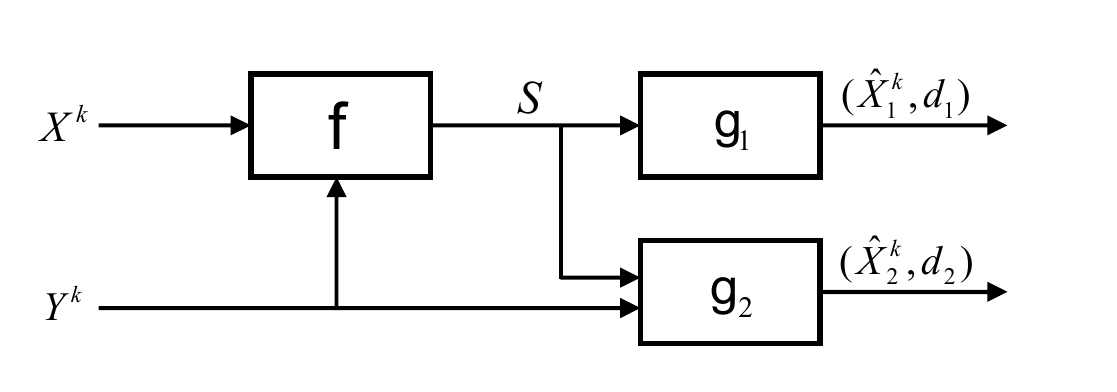
\includegraphics[width=0.85\linewidth]{fig/fig2.png}
  \caption{Kaspi 문제의 시스템 모형.}
\end{figure}

\subsubsection{Kaspi 문제}

Kaspi 문제의 모형은 그림~2와 같으며, 공통 부호기 $\ff$ 하나와 복호기 $\gg_i$ ($i=1,2$) 둘로 이루어진다.
부가 정보 $Y^k$는 $\gg_2$에서만 쓸 수 있다.
복호기 출력이 $\widehat{X}_i^k$ ($i=1,2$) 둘이므로, 서로 다른 왜곡 척도 두 개와 그에 대응하는 제약을 쓴다.
비점근 영역에서는 결합 초과 왜곡 확률
$P_{e,k}(d_1,d_2)\triangleq\P\left[\dd_1(X^k,\widehat{X}_1^k)>d_1 \text{ 또는 } \dd_2(X^k,\widehat{X}_2^k)>d_2\right]$
로 성능을 측정한다. 이 확률은 원천 분포와 부호책 분포를 모두 고려한다.
사실 [28]에서는 최적 부호의 성능을 평가하는 데 개별 초과 왜곡 확률을 썼다.
그러나 Zhou 등 [29]은 결합 초과 왜곡 확률이 개별 확률보다 여러 장점이 있다고 지적했다.
따라서 여기서는 결합 초과 왜곡 확률 기준에 기반한 결과에 집중한다.

[27]에서는 P2P $\dd$-기울인 정보를 Kaspi 문제의 $(\dd_1,\dd_2)$-기울인 정보로 확장했다.
$(\dd_1,\dd_2)$-기울인 정보의 핵심 성질 하나는, 원천과 부가 정보에 대한 기댓값이 율-왜곡 함수와 같다는 것이다. 즉 $R(P_{XY},d_1,d_2)=\E[\ttl_K(X,Y\mid d_1,d_2,P_{XY})]$이다.
Zhou 등은 $(\dd_1,\dd_2)$-기울인 정보의 이 성질과 Kostina 등의 단일 시행 역 논증 [89]을 바탕으로 Kaspi 문제의 역 한계를 유도했다 [27, Lemma 5].
달성 가능성 부분에서는 Kaspi 문제에 대한 형(type) 덮개 보조정리를 얻고, $(\dd_1,\dd_2)$-기울인 정보의 성질을 적절한 테일러 전개와 함께 활용했다.
Zhou 등은 Berry-Esséen 정리를 적용해 점근 근사를 유도했을 뿐 아니라, 대편차와 중편차를 이용해 DMS에 대한 오류 지수의 점근적 거동도 유도했다 [27, Sec.~III, Sebsec.~D].
여기서는 주로 Berry-Esséen 정리로 얻은 Kaspi 문제의 최적 2차 부호율을 소개한다.

\begin{figure}[t]
  \centering
  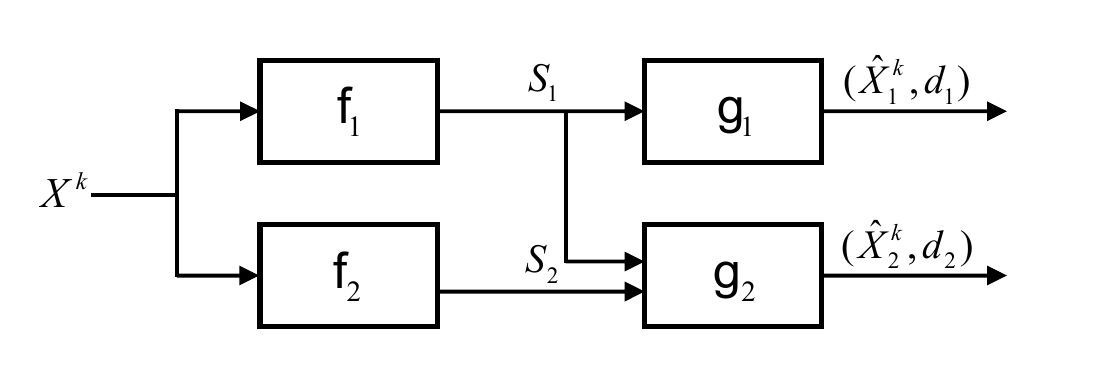
\includegraphics[width=0.85\linewidth]{fig/fig3.png}
  \caption{점진적 정밀화 문제의 시스템 모형.}
\end{figure}

Kaspi 문제의 왜곡-분산도 함수를 $V(d_1,d_2,P_{XY})$로 나타내자. 즉
\[
  V(d_1,d_2,P_{XY})=\Var\left[\ttl_K(X,Y\mid d_1,d_2,P_{XY})\right]
\]
이다.
부호율 $L$이 2차 $(d_1,d_2,\epsilon)$-달성 가능하다는 것은, 다음 두 조건을 만족하는 $(k,M)$-부호의 수열이 존재한다는 뜻이다.
\[
  \limsup_{k\to\infty}\frac{1}{\sqrt{k}}\left(\log M - k\,R(P_{XY},d_1,d_2)\right)\le L,
  \qquad
  \limsup_{k\to\infty}P_{e,k}(d_1,d_2)\le\epsilon.
\]
최적 2차 부호율은 이러한 달성 가능한 부호율 전체의 하한(infimum)으로 정의하고 $L^\star(d_1,d_2,\epsilon)$으로 나타낸다. 그 값은 다음과 같다.
\begin{equation}
  L^\star(d_1,d_2,\epsilon) = \sqrt{V(d_1,d_2,P_{XY})}\,Q^{-1}(\epsilon).
  \tag{16}
\end{equation}
덧붙여, 왜곡 수준 $(d_1,d_2)$에 따라 Kaspi 문제의 핵심 양 $\ttl_K(x,y\mid d_1,d_2,P_{XY})$는 다른 경우의 양으로 환원된다.
예를 들어 복호기 $\gg_2$를 없애면 Kaspi 문제는 통상적인 손실 원천 부호화 문제가 되고, $\ttl_K(x,y\mid d_1,d_2,P_{XY})$는 [10]의 $d_1$-기울인 정보로 환원된다.
마찬가지로 복호기 $\gg_1$을 없애면 부호기와 복호기 모두에서 부가 정보를 쓸 수 있는 경우가 되고, $\ttl_K(x,y\mid d_1,d_2,P_{XY})$는 [90]의 $d_2$-기울인 정보로 환원된다.

\subsubsection{점진적 정밀화}

점진적 정밀화 문제는 그림~3과 같다.
추가 복호기 하나가 두 부호기의 압축 출력에 동시에 접근한다 [88].
이 추가 복호기는 한 부호기에서만 정보를 받는 모형보다 원천 수열을 더 정밀하게 복원한다.
또한 점진적 정밀화 정식화는 다음 질문과 관련이 있다. 손실 압축의 최적성을 희생하지 않고도 전송을 중간에 끊었다가 특정 원천 수열을 더 잘 복원할 수 있는가 [30]?
Rimoldi는 [30]에서 임의의 왜곡 척도에 대해 DMS의 최적 율-왜곡 영역을 규명했다.
Effros는 이후 [31]에서 Rimoldi의 연구를 이산 정상 에르고딕 원천과 비에르고딕 원천으로 일반화했다.
Kanlis 등 [91]은 결합 초과 왜곡 기준 아래에서 오류 지수를 얻었고, Tuncel 등 [92]은 개별 초과 왜곡 기준을 다루었다.
No 등 [28]은 강한 점진적 정밀화 문제의 2차 부호율을 유도했다.
Zhou 등 [29]은 임의의 왜곡 척도를 지닌 DMS에 대해, 결합 초과 왜곡 기준 아래 점진적 정밀화 원천 부호화 문제의 최적 2차 부호율 영역과 중편차 상수를 유도했다.
이들은 이차 왜곡 척도를 쓰는 GMS도 다루었다. 이차 왜곡 척도 아래의 GMS는 점진적으로 정밀화 가능하므로 [88], 이 경우 결과가 특히 간단하다.

일반적인 DMS에서 율-분산도 행렬 $\mathbf{V}(R_1^\star,d_1,d_2\mid P_X)\succ 0$을 다음 2차원 확률벡터의 공분산 행렬로 두자.
\[
  \left[\,\ttl(X,d_1\mid P_X),\ \ttl(X,R_1^\star,d_1,d_2\mid P_X)\,\right]^T
\]
일정한 조건 아래에서 2차 부호율 영역은 [29, Theoremă11]에서 규명되었으며, 세 경우로 나뉜다\onote{``Theoremă11''은 조판 오류로, ``Theorem~11''로 읽는다. 문단 끝의 ``Theoremă6''도 ``Theorem~6''이다.}.
처음 두 경우에서는 부호의 부호율이 1차 한계 중 하나와 일정한 간격을 두고 떨어져 있으므로, 2차 거동을 일변량 가우스 분포로 포착할 수 있다.
반면 셋째 경우에서는 부호가 두 1차 한계에서 정확히 동작하므로, 2차 거동을 포착하려면 이변량 가우스 정식화가 필요하다.
이 결과는 Tan 등 [93, Theoremă6]의 논증에 따라 율-분산도 행렬이 양의 정부호인 경우와 계수 부족(rank-deficient)인 경우 모두에 성립한다.

% 3장 채널 부호화 (원문 pp. 20--31, 식 (17)--(33), 그림 4--5)
\section{채널 부호화}

채널 부호화의 기본 과제는 잡음이 있는 채널로 $M$개의 메시지를 보내되, 수신단에서 이들을 신뢰성 있게 구별할 수 있게 하는 것이다. 이 장에서는 채널 부호화의 정보이론적 근본 한계에 관한 최근 진전을 살펴본다. 특히 P2P 채널, 다중 접속 채널, 대규모 접속 채널에 초점을 둔다.

\subsection{P2P 채널}

\subsubsection{핵심 지표}

Shannon이 세운 통신의 기본 틀 [8]은 채널 부호화를 다음 네 가지 핵심 구성 요소로 정식화한다.
1) 사전에 알려지지 않은 메시지. 이 메시지는 집합 $\{1,\dots,M\}$ 위에서 균등한 확률변수 $W$로 모형화한다.
2) 부호기 $\ff:\{1,\dots,M\}\to\mathcal{X}^n$. 부호기는 메시지 $W$를 길이 $n$인 부호어 $X^n$으로 사상한다.
3) 채널. 채널은 입력 $x^n\in\mathcal{X}^n$과 출력 $y^n\in\mathcal{Y}^n$을 잇는 무작위 변환의 수열 $P_{Y^n|X^n}$으로 모형화한다.
4) 복호기 $\gg:\mathcal{Y}^n\to\{1,\dots,M\}$. 복호기는 채널 출력 $Y^n$을 바탕으로 메시지의 추정값 $\widehat{W}$를 내놓는다.

$(n,M,\epsilon)$-부호란 부호 길이가 $n$이고 부호책 크기가 $M$이며, 복호 오류 확률이 $\epsilon$ 이하임을 보장하는 부호기-복호기 쌍 $(\ff,\gg)$를 말한다. 흔히 쓰는 오류 제약은 두 가지로, 평균 오류 확률 제약과 최대 오류 확률 제약이다. 각각 다음과 같다.
\begin{align}
P_{\mathrm{e,ave}} &= \P\bigl[\widehat{W}\neq W\bigr]\le\epsilon, \tag{17}\\
P_{\mathrm{e,max}} &= \max_{1\le j\le M}\P\bigl[\widehat{W}\neq W \,\big|\, W=j\bigr]\le\epsilon. \tag{18}
\end{align}
율(rate)은 $R\triangleq\frac{\log M}{n}$으로 정의하며, 단위는 채널 사용당 비트이다. 부호 길이 $n$과 목표 오류 확률 $\epsilon$이 주어졌을 때의 최대 데이터율을 나타내는 근본 한계 $R^\star(n,\epsilon)$은 다음과 같이 정의한다.
\begin{equation}
R^\star(n,\epsilon)\triangleq\sup\left\{R:\exists\,(n,M,\epsilon)-\text{code}\right\}. \tag{19}
\end{equation}
마찬가지로, 달성할 수 있는 가장 작은 오류 확률은 다음과 같이 정의한다.
\begin{equation}
\epsilon^\star(n,R)\triangleq\sup\left\{\epsilon:\exists\,(n,2^{nR},\epsilon)-\text{code}\right\}. \tag{20}
\end{equation}
\onote{본문은 ``가장 작은'' 오류 확률이라고 하므로, 식 (20)의 $\sup$은 $\inf$여야 맞다. 여기서는 원문대로 옮겼다.}

\subsubsection{고전적 점근 결과}

Shannon의 선구적 연구 [8]는 $(n,\epsilon)$ 쌍이 주어졌을 때 $R^\star(n,\epsilon)$을 분석하는 이론적 토대를 놓았다. Shannon이 관찰한 놀라운 사실은, 부호 길이 $n$이 무한대로 가고 오류 확률 $\epsilon$이 0으로 가면 $R^\star(n,\epsilon)$을 점근적으로 다룰 수 있게 된다는 것이다. 이때 $R^\star(n,\epsilon)$의 점근 극한을 채널 용량 $C$라 한다. 즉,
\begin{equation}
C=\lim_{\epsilon\to0}\lim_{n\to\infty}R^\star(n,\epsilon). \tag{21}
\end{equation}
이 식은 부호 길이가 충분히 길기만 하면 용량보다 낮은 어떤 율에서도 오류 없는 전송이 가능함을 보여 준다. 무기억 채널 $P_{Y|X}$의 채널 용량 $C$는 다음과 같이 쓸 수 있다 [8], [66, Sec.~7].
\begin{equation}
C=\sup_{P_X}I(X;Y), \tag{22}
\end{equation}
여기서 $I(X;Y)$는 $X$와 $Y$ 사이의 단일 문자 상호 정보량이고, 상한은 모든 입력 분포에 대해 취한다. $\epsilon>0$을 고정하고 $n\to\infty$로 보낼 때 $R^\star(n,\epsilon)$의 극한을 $\epsilon$-용량 $C_\epsilon$이라 한다. 즉,
\begin{equation}
C_\epsilon=\lim_{n\to\infty}R^\star(n,\epsilon). \tag{23}
\end{equation}

율 $R$을 고정하면, $\epsilon^\star(n,R)$의 점근적 거동은 신뢰도 함수 $E(R)$이 결정한다. 즉,
\begin{equation}
E(R)=\liminf_{n\to\infty}-\frac{\log\epsilon^\star(n,R)}{n}. \tag{24}
\end{equation}
율 $R$이 용량 $C$를 넘으면 통신은 신뢰할 수 없고, 이때 $E(R)=0$이다. 반면 $R<C$로 제한하면 오류 확률은 지수 $E(R)>0$으로 지수적으로 감소할 수 있다.

\subsubsection{비점근 한계}

고전 정보이론은 무한한 부호 길이, 무한한 페이로드 크기, 사라지는 오류 확률 가운데 일부 또는 전부를 가정한다. 그래서 짧은 부호 길이와 짧은 패킷을 쓰고, 작지만 무시할 수 없는 오류 확률을 요구하는 실제 통신 시스템의 근본 한계는 규명하지 못한다. 이 문제를 피하고자 여러 연구가 유한 부호 길이 정보이론에 집중해 왔다. 유한 부호 길이 영역에서는 단순한 이진 대칭 채널이나 이진 소거 채널에서조차 최대 율 $R^\star(n,\epsilon)$을 정확히 계산하기가 계산상 불가능하다. 이 때문에 연구자들은 달성 가능성 쪽과 역 쪽 모두에서 촘촘하면서도 계산 가능한 한계를 개발하게 되었다. 아래에서는 몇 가지 비점근 한계와 그 유도에 쓰인 핵심 아이디어를 살펴본다.

\paragraph{1) 달성 가능성 한계}
Feinstein [94]과 Shannon [95]은 각각 최대 부호화와 무작위 부호화 아이디어에 기초하여 $R^\star(n,\epsilon)$에 대한 유한 부호 길이 달성 가능성 한계(곧 하한)를 세웠다. 무작위 부호화 아이디어에서는 어떤 분포로부터 부호책을 무작위로 구성한 뒤, 앙상블의 여러 실현에 걸쳐 오류 확률을 평가한다. 이로써 평균 오류 확률 제약 아래에서 부호가 존재함을 증명한다. 최대 부호화 방식에서는 최대 오류 확률 제약을 어기게 될 때까지 부호어를 하나씩 차례로 덧붙인다. 문헌에 있는 달성 가능성 한계는 거의 모두 이 두 아이디어를 바탕으로 한다. 한계 사이의 차이는 주로 복호 규칙(전형성 복호, 최대 우도 복호, 문턱값 복호 등)과 오류 분석 기법에 있다. 예를 들어 Polyanskiy, Poor, Verdú [11]는 $R^\star(n,\epsilon)$에 대해 해석적으로 다루기 쉽고 비점근적으로도 날카로운 달성 가능성 한계를 여럿 유도했는데, 의존성 검정(DT, dependence-testing) 한계와 $\kappa\beta$ 한계가 그 예이다. 이러한 달성 가능성 한계를 유도하는 핵심 원리는 무작위/최대 부호화와 가설 검정이다. $R^\star(n,\epsilon)$에 대한 한계와 별도로, Gallager [96]는 신뢰도 함수 분석에 더 알맞은 달성 가능성 한계를 유도했다(최근 개관은 [97] 참고). 또한 [32]에서는 점근적 황금 공식(golden formula)과 비점근 $\beta\beta$ 한계 사이의 관계를 규명했다. 도청 채널의 비점근 근본 한계는 [98]에서 탐구했다.

위의 한계는 전력 제약이 있는 시스템으로 자연스럽게 일반화할 수 있다. 입력 분포는 유한 부호 길이 성능을 크게 좌우한다. 대부분의 부호어 전력을 쓸 수 있는 최대 전력 예산 근처에 모으면 성능이 크게 좋아진다. 그래서 [11]과 [99]는 1차 최적인 i.i.d.\ 가우스 부호어 대신 전력 껍질에서 뽑은 부호어의 입력 앙상블을 썼다. Gallager는 얇은 껍질 안에 놓인 절단 가우스 분포로 부호어를 생성하는 방법을 제안했다 [100]. 아울러 위의 결과는 되먹임이 있는 채널로도 일반화할 수 있다. 구체적으로, Polyanskiy 등 [33]은 오류 확률이 고정되고 평균 복호 시간이 유한할 때 달성할 수 있는 최대 부호책 크기에 대한 비점근 한계를 유도했고, 이 한계는 [34]에서 더 개선되었다. [34]의 저자들은 또한 평균 전력 제약이 있는 이산 무기억 채널과 AWGN 채널(가산 백색 가우스 잡음 채널)에 대해, 바탕에 있는 채널 매개변수를 몰라도 되는 범용 가변 길이 되먹임 부호를 개발했다.

\paragraph{2) 역 한계}
문헌에는 역 한계가 많이 세워져 있다. Fano 부등식은 $R^\star(n,\epsilon)$에 대한 약한 역 한계(곧 상한)를 증명하는 고전적 도구이다 [66, Sec.~7.9]. 한편 Wolfowitz [101]는 이산 무기억 채널에 대한 강한 역 한계를 세웠다. [102]의 저자들은 신뢰도 함수 분석에 알맞은 구 채우기 역 한계를 유도했다. Verdú와 Han [103]은 정보 스펙트럼(information spectrum)에 기초한 역 한계를 세웠는데, 이 한계는 임의의 무작위 변환에 대해 성립한다. 이후 Polyanskiy, Poor, Verdú는 가설 검정과 여러 데이터 처리 부등식에 기초하여 메타 역정리 한계라는 일반적인 역 한계를 유도했다 [65]. [65, Sec.~2.7.3]과 [35]에서는 대부분의 역 결과를 이 메타 역정리 한계로부터 되찾을 수 있음을 보였다.

\paragraph{3) 수치 결과}
그림~4는 P2P AWGN 채널에서 최대 전력 제약 아래 $R^\star(n,\epsilon)$에 대한 여러 달성 가능성 한계와 역 한계를 비교한다. 비점근 한계와 점근 용량 사이의 간격이 크다는 점에서, $n$과 $\log M$이 작은 짧은 패킷 통신에 유한 부호 길이 정보이론을 적용하는 일이 얼마나 중요한지 드러난다. 비점근 달성 가능성 한계 가운데 Shannon 한계가 가장 촘촘하지만, AWGN에 특화된 설정에만 쓸 수 있다. $\kappa\beta$ 한계는 Shannon 한계보다 조금 느슨하지만, 점근 분석에서 계산상 더 다루기 쉽고 더 일반적이다. Feinstein 한계는 $\kappa\beta$ 한계보다 느슨하다. $\kappa\beta$ 한계는 Gallager 한계와 비교하면 $n$이 큰 영역에서는 더 촘촘하지만 $n$이 작을 때는 더 느슨하다. 그림~4에는 저복잡도 신뢰 전파(belief propagation) 기반 복호기를 쓰는 다중 에지(multi-edge) 저밀도 패리티 검사(LDPC, low-density parity-check) 부호의 성능도 함께 나와 있다. 이 실용 기법을 용량과 비교하면, $n$이 커질수록 기법이 최적에 가까워짐을 알 수 있다. 그러나 이 기법과 유한 부호 길이 한계 사이의 간격은 부호 길이와 거의 무관하다. 이 불일치는 부호 설계를 평가하는 패러다임이 바뀌어야 함을 보여 준다. 즉 짧은 패킷 통신의 성능을 정확히 평가하려면 점근 지표를 넘어 유한 부호 길이 정보이론을 받아들여야 한다.

차세대 채널 부호화는 6G의 엄격한 요구 사항을 만족해야 할 뿐 아니라, 이미 빽빽한 기저대역 칩에 부담을 더 얹지 않도록 하위 호환성도 갖추어야 한다. 이런 배경에서 [104]의 저자들은 6G 통신을 위한 후보 채널 부호를 검토하고, LDPC와 폴라(polar) 틀에 기초한 차세대 채널 부호를 탐구했다. [104]에서는 폴라 유사 성분을 지닌 일반화 LDPC(GLDPC-PC, generalized LDPC with polar-like component) 부호라는 새로운 개념을 도입했다. 이 부호에서는 폴라 성분이 변수 노드로 넘기는 연판정 정보(soft information)를 연출력 연속 제거 목록(SO-SCL, soft-output successive cancellation list) 복호기 [105]로부터 효율적으로 추출한다. 그런데 연속 제거 목록 복호는 본질적으로 순차적이어서 SO-SCL 복호기의 복호 지연이 크다. 이를 고려하여 [106]의 저자들은 노드 기반 고속 복호를 SO-SCL 틀에 결합한 연출력 고속 SCL(SO-FSCL) 복호기를 제안했다. 더 자세한 내용은 [104, 105, 106]을 참고하라.

\begin{figure}[t]
\centering
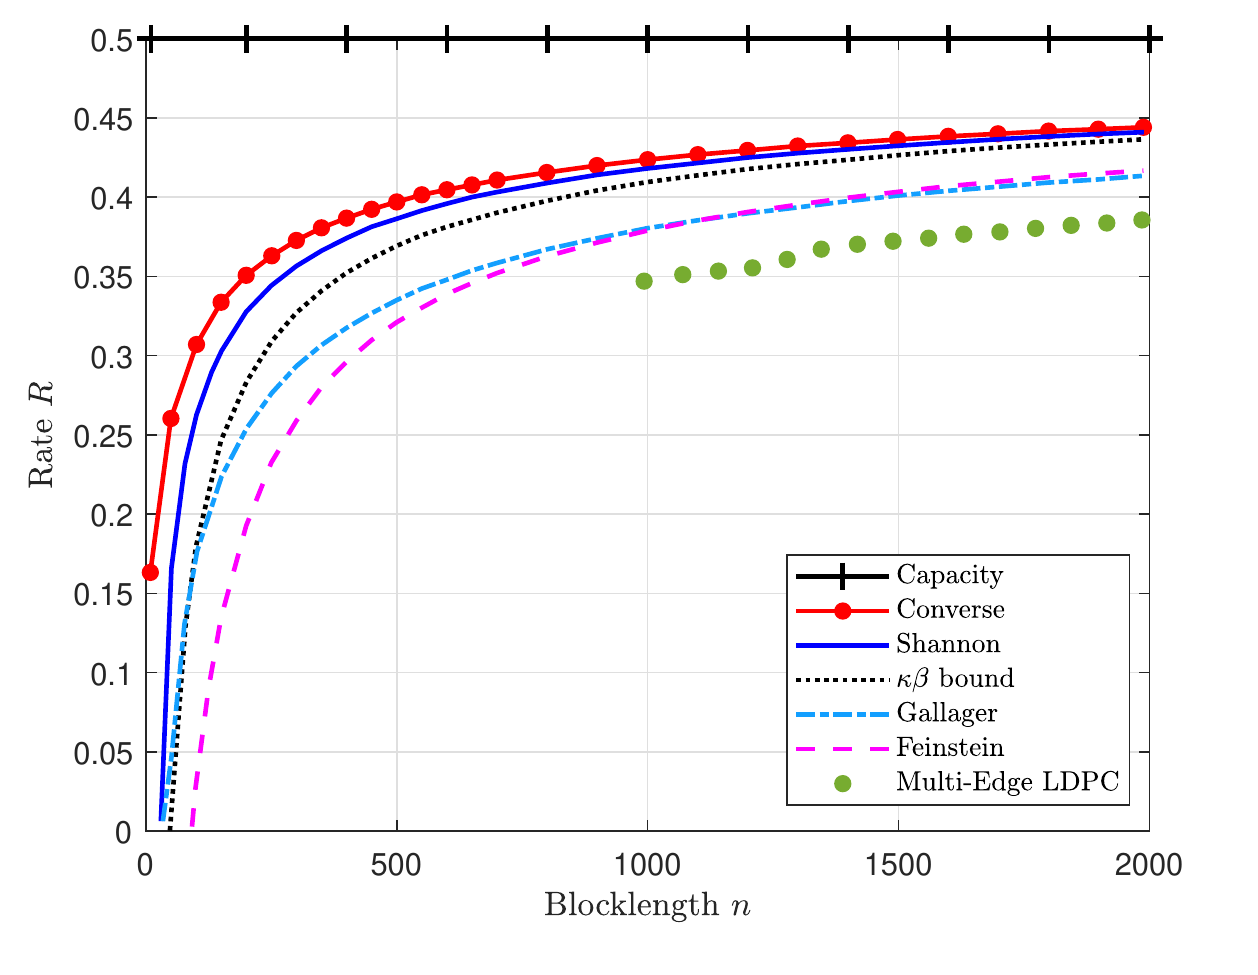
\includegraphics[width=0.85\linewidth]{fig/fig4.png}
\caption{SNR $=0$\,dB, $\epsilon=10^{-3}$인 AWGN 채널에서 P2P 통신의 이론적 한계와 다중 에지 LDPC 알고리즘.}
\end{figure}

\subsubsection{근사}

무선 통신 시스템 설계에 공학적 통찰을 주려면, 상한과 하한보다 계산 복잡도가 낮으면서 다루기 쉬운 $R^\star(n,\epsilon)$의 근사를 개발하는 일이 매우 중요하다. 이를 위한 분석 기법으로는 서로 보완적인 세 가지, 곧 CLT, 대편차(LD), 중편차(MD, moderate deviations)가 있으며, 아래에서 차례로 소개한다.

Polyanskiy, Poor, Verdú [11]는 Strassen [73]의 고전적 전개 결과를 바탕으로, CLT 영역에서는 채널의 2차 통계량인 채널 분산도를 도입하면 최대 부호율 $R^\star(n,\epsilon)$을 촘촘하게 근사할 수 있음을 보였다. 채널 분산도는 다음과 같이 정의한다 [11, Def.~1].
\begin{equation}
V=\lim_{\epsilon\to0}\lim_{n\to\infty}n\left(\frac{C-R^\star(n,\epsilon)}{Q^{-1}(\epsilon)}\right)^{2}. \tag{25}
\end{equation}
용량 $C$가 양수인 여러 채널에서 최대 부호율 $R^\star(n,\epsilon)$은 정규 근사 [11]로 촘촘하게 근사된다.
\begin{equation}
R^\star(n,\epsilon)=C-\sqrt{\frac{V}{n}}\,Q^{-1}(\epsilon)+O\!\left(\frac{\log n}{n}\right). \tag{26}
\end{equation}
이 근사에 따르면, 부호 길이 $n$에서 오류 확률을 $\epsilon$ 이하로 보장하려면 율 면에서 (채널 용량에 비해) $\frac{1}{\sqrt{n}}$에 비례하는 손실을 치러야 한다. 부호 길이 $n$이 무한대로 가면 이 율 손실은 0으로 간다.

신호 대 잡음비(SNR, signal-to-noise ratio)가 $P$인 AWGN 채널에서 $C$와 $V$는 다음과 같다 [11, Theorem~54].
\begin{align}
C &= \frac{1}{2}\log(1+P), \tag{27}\\
V &= \frac{P}{2}\,\frac{(2+P)}{(1+P)^2}\log^2 e. \tag{28}
\end{align}
[11]의 결과는 여러 무선 통신 채널로 일반화되었다. 페이딩 계수가 한 부호어 동안 변하지 않는 MIMO 준정적 페이딩 채널에서는, [36, Theorem~3]에 제시된 페이딩 분포에 대한 완만한 조건 아래 채널 분산도가 0임이 증명되었다. 즉 다음이 성립한다 [36].
\begin{equation}
R^\star(n,\epsilon)=C_\epsilon+O\!\left(\frac{\log n}{n}\right). \tag{29}
\end{equation}
채널 분산도는 에르고딕 페이딩 채널에 대해서도 연구되었다. 구체적으로, 수신단에 채널 상태 정보(CSI, channel state information)가 알려진 단일 입력 단일 출력(SISO, single-input single-output) 정상 페이딩 채널의 분산도는 [37]에서 유도되었다. 이 결과는 [107]에서 SISO 블록 무기억 페이딩 채널로, [38]에서 다중 입력 다중 출력(MIMO, multiple-input multiple-output) 블록 무기억 페이딩 채널로 확장되었다. 안테나 수가 부호 길이에 비례하여 늘어나는 점근적 에르고딕 설정에 대해서는, [39]가 MIMO 준정적 레일리(Rayleigh) 페이딩 채널의 2차 부호율에 대한 상한과 하한을 제시했다. You 등 [40]은 대규모 MIMO 시스템에서 달성 가능한 율의 상한에 대한 닫힌 형태의 근사를 다음과 같이 유도했다.
\begin{equation}
\frac{R^\star(n,\epsilon)}{m}\le\log(1+P)-\sqrt{\frac{1}{nm}}\,Q^{-1}(\epsilon), \tag{30}
\end{equation}
여기서 $m$은 공간 자유도이다. 이 식에서 $mn$ 값을 고정하면 Hz당·안테나당 평균 데이터율이 변하지 않음을 알 수 있다. 이는 $n$과 $m$이 어느 정도 서로 맞바꿀 수 있는 관계임을 뜻하며, 따라서 안테나 수를 늘리면 필요한 부호 길이를 크게 줄일 수 있다. 이어서 [108]에서는 시공간 부호화에 대한 명시적 성능 한계를 유도했다. 시공간 부호화는 6G 시스템에서 지연을 줄이는 핵심 수단으로 떠오르고 있다 [109].

LD 영역에서 오류 확률, 율, 부호 길이 사이의 상충 관계를 분석하는 연구는 1960년 Gallager의 선구적 연구 [96]까지 거슬러 올라간다. 이 연구에서는 용량보다 엄격히 낮은 율 $R$을 고정하면 오류 확률 $\epsilon^\star(n,R)$이 $n$에 대해 지수적으로 감소함을 증명했다. 즉,
\begin{equation}
\epsilon^\star(n,R)=\exp\bigl(-n(E(R)+o(1))\bigr). \tag{31}
\end{equation}

CLT형 근사와 LD형 근사는 서로 다른 경우에 지배적이다. $\epsilon$이 클 때(곧 $R$이 용량에 가까울 때)는 CLT 근사가, $\epsilon$이 작을 때(곧 $R$이 용량보다 훨씬 작을 때)는 LD 근사가 지배적이다. MD 분석은 이 두 영역의 사이를 다룬다 [41, 42]. MD 분석에 따르면 오류 확률은 $n$에 대해 준지수적으로(subexponentially) 감소하고, 달성 가능한 최대 율은 $1/\sqrt{n}$보다 느리게 채널 용량에 수렴한다. 구체적으로 MD 분석에서 다음 근사를 얻는다.
\begin{equation}
\epsilon^\star(n,C-\delta_n)\approx Q\!\left(\sqrt{\frac{n}{V}}\,\delta_n\right)\approx\exp\!\left(-\frac{n\delta_n^2}{2V}\right), \tag{32}
\end{equation}
여기서 $n\to\infty$일 때 $\delta_n>0$, $\delta_n\to0$, $n\delta_n^2\to\infty$이다. [110]에서는 MD 분석에 기초하여 최대 율에 대한 3차 근사를 유도했다.

\subsection{다중 접속 채널}

여러 사용자가 동시에 시스템에 접속하는 다중 접속 채널(MAC, multiple access channel)은 무선 통신망의 기초 모형이다. 사용자 수 $K$가 고정된 가우스 MAC에서 점근 용량 영역은 다음을 만족하는 모든 달성 가능한 율 순서쌍 $(R_1,R_2,\dots,R_K)$의 볼록 껍질로 정의한다.
\begin{equation}
\sum_{i\in S}R_i\le C\!\left(\sum_{i\in S}P_i\right),\quad\forall S\subseteq\{1,2,\dots,K\}, \tag{33}
\end{equation}
여기서 $P_i$는 사용자 $i$의 SNR이고, $C(\cdot)$는 P2P 가우스 채널의 Shannon 용량이다. 이 영역은 $2^K-1$개의 부등식으로 둘러싸인 $K$차원 다면체로, 개별 율과 그 합 사이의 상충 관계를 반영한다. $K=2$이면 용량 영역은 오각형으로 단순해진다 [111].

위의 용량 분석은 부호 길이가 무한하다는 가정에 기댄다. $K\ll n$을 만족하는 유한 부호 길이 MAC에 대해, MolavianJazi와 Laneman [43], 그리고 Huang과 Moulin [44]은 P2P 채널의 유한 부호 길이 결과를 송신기가 둘인 MAC으로 일반화했다. 이들의 유한 부호 길이 결과는 전역 분산도 행렬(global dispersion matrix)에 기초한다. Haim 등 [45]이 논의했듯이, 관심 있는 대부분의 경우에 분산도 행렬의 비대각 성분은 성능을 규명하는 데 근본적인 역할을 하지 않는다. 율 영역 경계면 위에서 모서리가 아닌 점에 다가갈 때 특히 그렇다. 이 점에 착안하여 [46, 47]은 다중 접속 채널의 국소(local) 2차 점근 해석을 연구했다.

\subsection{대규모 무작위 접속 채널}

\subsubsection{정보이론적 한계}

사물인터넷(IoT, Internet of Things) 응용이 빠르게 늘어나면서, 초대규모 기계형 통신(umMTC, ultra-massive machine-type communication)은 차세대 무선 시스템에서 핵심적인 위치를 차지하게 되었다. 기존 MAC에서는 사용자 수가 대개 고정되어 있고 부호 길이보다 훨씬 작다. 반면 umMTC에서는 사용자 수가 부호 길이와 비슷하거나 더 크며, 그 가운데 일부만 활성 상태로 짧은 패킷(예를 들어 수백 비트)을 기지국(BS, base station)에 보낸다. 이처럼 많은 사용자에게 제한된 채널 사용 횟수와 엄격한 에너지 제약 아래 효율적이고 신뢰성 있는 무작위 접속을 제공하는 것이 umMTC의 핵심 과제이다 [112, 113, 114]. 대규모 무작위 접속에는 서로 다른 두 패러다임이 등장했다. 1) 개별 부호책 기반 대규모 무작위 접속. 각 사용자에게 고유한 부호책을 할당하여 활성 사용자 검출과 메시지 복호에 쓴다. 2) 공통 부호책 기반 대규모 무작위 접속. 사용자가 하나의 공통 부호책을 공유하고, 수신기는 전송된 메시지를 특정 사용자와 연결하지 않은 채 순서에 무관한(permutation-invariant) 목록으로 복원한다. 두 번째 방식은 무출처 무작위 접속(URA, unsourced random access)이라고도 한다 [48]. 대규모 무작위 접속의 근본 한계를 규명하는 일은 매우 중요하다.

[115]에서는 방대한 사용자 집단을 규명하기 위해 다수 접속 채널(MnAC, many-access channel)이라는 모형을 제안했다. 이 모형에서는 사용자 수가 부호 길이와 함께 늘어난다. 후속 연구는 선형 스케일링 가정 아래 이 모형을 채택했다. 그러나 [115]는 유한한 비트당 에너지, 페이로드 크기, 부호 길이 같은 실제 제약을 간과했다. 이를 보완하고자 일부 연구는 부호 길이는 무한하지만 페이로드 크기와 비트당 에너지는 유한한 영역을 다루었으며 [116, 117, 118], 이때 [48]에서 제안한 사용자별 오류 확률(PUPE, per-user probability of error) 기준을 채택했다. 특히 Zadik 등 [116]과 Kowshik 등 [117]은 선형 스케일링 MnAC 모형에서 각 사용자에게 개별 부호책을 할당하고 기지국에 안테나가 하나뿐이라고 가정했다. 그리고 각각 AWGN 채널과 준정적 페이딩 채널에서 필요한 최소 비트당 에너지에 대한 달성 가능성 한계와 역 한계를 유도했다. 그 결과 사용자 밀도가 낮을 때는 다중 사용자 간섭(MUI, multi-user interference)을 거의 완벽하게 제거할 수 있음을 밝혔다.

지연에 민감한 응용에서는 유한 부호 길이 분석이 필요하다. URA에 대한 비점근 한계는 가우스 채널에 대해 [48]에서, 레일리 페이딩 채널에 대해 [49]에서 유도되었다. [50]의 저자들은 [48]의 결과를, 각 사용자가 동일한 재생 과정(renewal process)에 따라 독립적이고 비동기적으로 패킷을 생성하는 경우로 확장했다. 이 연구는 모두 활성 사용자 수를 미리 안다는 가정에 기댄다. 그러나 대규모 무작위 접속 채널에서 사용자는 대개 간헐적이거나 버스트(bursty)한 통신 패턴을 보이고 승인(grant) 없이 망에 접속한다. 그 결과 활성 사용자 수가 변동하고 불확실해진다. 이 문제를 다루기 위해 [51]은 활성 사용자 수가 무작위이고 알려지지 않은 가우스 채널에서 대규모 무작위 접속을 고려했고, 미검출 확률과 오경보 확률에 대한 비점근 한계를 유도했다.

위의 이론적 결과는 모두 기지국에 안테나가 하나뿐인 상황에서 세운 것이다. 활성 사용자 검출에 대해서는 [119]에서 다음을 증명했다. 채널 사용 횟수가 $n$이고 안테나 배열 크기 $L$이 $K_a/L=o(1)$을 만족할 만큼 충분히 크면, $\frac{K_a}{K}=\Theta(1)$이라는 조건 아래 기지국은 잠재 사용자 $K$명 가운데 최대 $K_a=O(n^2)$명의 활성 사용자를 검출할 수 있다. 활성 사용자 수가 부호 길이에 선형으로만 늘어날 수 있는 단일 안테나 시스템에 비하면 크게 나아진 결과이다. 다중 수신 안테나의 큰 잠재력에 착안하여, [52]의 저자들은 MIMO 준정적 레일리 페이딩 채널에서 개별 부호책을 쓰는 대규모 무작위 접속에 대해 비점근 달성 가능성 한계와 역 한계를 유도했다. 이 결과를 바탕으로 수신단의 CSI가 알려진 경우와 알려지지 않은 경우 모두에서 부호 길이, 페이로드 크기, 사용자 밀도, 수신 안테나 수, 오류 확률 사이의 근본적 상충 관계를 규명했다. [52]에서는 CSI를 모르는 경우 PUPE 기준 아래, 수신 안테나 수가 $L=\Theta(n^2)$이고 송신 전력이 $P=\Theta\bigl(\frac{1}{n^2}\bigr)$이면 최대 $K=O(n^2)$명의 사용자를 신뢰성 있게 지원할 수 있음을 증명했다. CSI를 아는 경우에는 완만한 조건 아래, PUPE 요구 사항이 만족될 필요충분조건이 $\frac{nL\ln KP}{K}=\Omega(1)$이다. 이 조건은 대규모 IoT 응용에서 MIMO 기술이 저비용·저지연 통신을 가능하게 할 잠재력이 있음을 보여 준다. 또한 특정 조건에서는 비트당 에너지가 유한할 수 있고 심지어 0에 가까워질 수도 있음을 보였는데, 이는 에너지 자원이 제한된 실제 시스템에 매우 중요하다. 아울러 MIMO 채널에서 URA의 근본 한계는 [53]과 [54]에서 탐구되었다. 두 연구는 각각 활성 사용자 수를 아는 경우와 모르는 경우에 대한 유한 부호 길이 한계를 세웠다.

\begin{figure}[t]
\centering
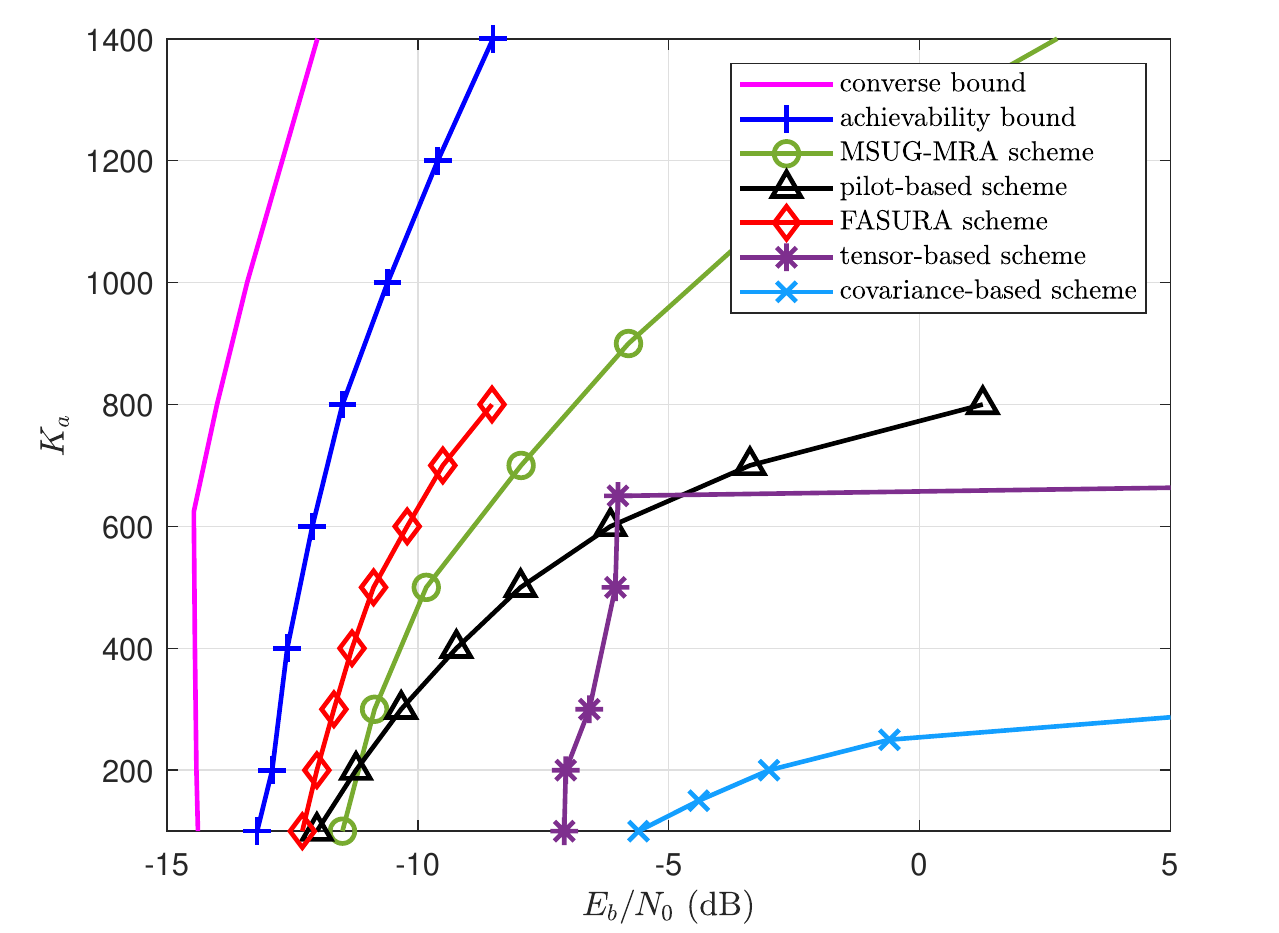
\includegraphics[width=0.85\linewidth]{fig/fig5.png}
\caption{MIMO 준정적 페이딩 채널에서 URA의 기존 기법과 이론적 달성 가능성 한계 및 역 한계의 비교. $K_a$는 고정되어 있고 알려져 있다고 가정하며, $n=3200$, $J=100$비트, $L=50$, $\epsilon_{\mathrm{MD}}=\epsilon_{\mathrm{FA}}=0.025$인 경우이다.}
\end{figure}

\subsubsection{실용 기법과의 비교}

앞에서 세운 유한 부호 길이 한계는 실용 기법을 평가하는 이론적 기준점이 된다. 그림~5에서는 [53]에서 유도한 MIMO 준정적 페이딩 채널의 URA에 대한 유한 부호 길이 달성 가능성 한계와 역 한계(구 위에 균등하게 분포한 부호어 사용)를, [119, 120, 121, 122, 123]에서 제안한 기존 최신 기법과 비교한다. 설정은 부호 길이 $n=3200$, 페이로드 크기 $J=100$비트, 기지국 안테나 수 $L=50$, 목표 미검출 확률과 오경보 확률 $\epsilon_{\mathrm{MD}}=\epsilon_{\mathrm{FA}}=0.025$이다. 최신 기법의 핵심 구현 사항은 다음과 같다. MSUG-MRA 기법은 [120, Fig.~4]와 같이 평가한다. 이 기법은 $n$을 $S$개의 슬롯으로 나누는 슬롯 구조를 쓴다. 각 활성 사용자는 슬롯 하나를 무작위로 고른다. 그 슬롯에서 전송하는 $J$비트 메시지는 $D$개의 직교 파일럿 구간(각 $B_p$비트)과 $J-DB_p$비트의 부호화 구간으로 나뉘며, $G$개의 서로 다른 인터리버-전력 그룹 할당으로 성능을 높인다. 파일럿 기반 기법은 [121, Fig.~7]과 같이 평가한다. 이 기법은 데이터를 각각 16비트와 84비트인 두 부분으로 나눈다. 첫 부분에는 길이 1152의 ``파일럿''을 쓰고, 둘째 부분은 길이 2048의 폴라 부호로 부호화한다. FASURA 기법은 [122, Fig.~4]와 같이 평가하며, 파일럿 기반 기법과 마찬가지로 메시지를 두 부분으로 나눈다. [121]과 다른 점은 길이 $L=9$인 확산 수열을 쓴다는 점, 활성 수열을 검출하는 방법, 그리고 채널/기호 추정 기법이다. 텐서 기반 기법은 [123]과 같이 평가한다. 이 기법은 BCH 외부 부호와 함께 텐서 서명 $(8,5,5,4,4)$를 쓰며, 오류 확률 $\epsilon=0.1$을 허용한다. 공분산 기반 기법은 [119]에서 제안되었다. 이 기법은 16슬롯 프레임을 쓰는데, 각 슬롯은 길이가 200이고, 트리 부호 패리티 프로파일 $[0,7,8,8,9,\dots,9,13,14]$에 따른 15비트를 포함한다. 그림~5에서 보듯 기존 기법은 $K_a$가 작을 때는 경쟁력 있는 에너지 효율을 유지한다. 그러나 $K_a$가 커질수록 성능이 더 많이 떨어지고, 이론적 한계에 비해 더 높은 비트당 에너지 $E_b/N_0$를 요구한다. 따라서 $K_a$가 큰 경우에는 더 진보하고 에너지 효율이 높은 기법 설계가 필요하다.

% ===== Part D: 4. 결합 원천-채널 부호화 / 5. 미해결 문제 / 6. 결론 (원문 31–37쪽) =====
\section{결합 원천-채널 부호화}

먼저 JSCC의 시스템 모형을 그림~6에 나타냈다. 부호기의 입력과 복호기의 출력은 길이 $k$인 벡터 $S^k$와 $Z^k$이다. 길이 $n$인 벡터 $X^n$과 $Y^n$은 각각 잡음 채널의 입력과 출력이다. JSCC의 부호율은 $\frac{k}{n}$으로 정의한다. 점근 영역에서 초과 왜곡 확률을 0으로 보내면, 달성 가능한 최대 JSCC 부호율은 $\frac{C}{R(d)}$이다. 여기서 $C$는 \emph{채널 용량}이고, $R(d)$는 미리 정한 평균 왜곡 제약 $d$ 아래의 \emph{율-왜곡 함수}이다. 이것이 [75]와 [66]의 원천-채널 분리 정리가 주는 고전적 결과이다. 다시 말해 점근 영역에서는 최적의 원천 부호와 채널 부호를 따로 설계한 뒤 이어 붙이기만 해도 점근적 근본 한계에 도달한다. 그러나 비점근 영역에서는 SSCC가 매우 느슨한 비점근 한계밖에 주지 못한다. 반면 JSCC 설계는 유한 부호 길이에서 상당한 이득을 낸다 [12]. 이는 두 설계 방식의 이론적 한계가 서로 다르며, 유한 부호 길이 영역에서 연구가 더 필요하다는 뜻이다.

Csiszár [55]는 JSCC의 오류 지수가 SSCC의 오류 지수보다 크다는 것을 증명했다. 평균 왜곡 기준 아래의 이산 원천-채널 쌍에 대해서는 Pilc [124, 56]가, 평균 제곱 오차 제약 아래에서 가우스 원천을 이산 채널로 전송하는 문제에 대해서는 Wyner [125, 57]가 비점근 한계를 얻었다. Csiszár는 [58]에서 그래프 이론적 JSCC 모형의 비점근 근본 한계도 유도했다. 거의 무손실인 JSCC 설정에서는 Campo 등 [126]이 유한 부호 길이 무작위 부호화 한계를 여럿 제시했다. 이어서 Wang 등 [59]은 원천과 채널의 알파벳이 유한한 경우에 JSCC의 분산도를 구했다. 끝으로 Kostina 등 [12]은 JSCC에 대한 새로운 일반적 달성 가능성 한계와 역 한계를 유도하고, 가우스 근사를 분석했으며, 여러 경우에 대한 결과를 얻었다. 이하에서는 JSCC의 근본 한계에 관한 주요 결과와 그 바탕에 있는 기본 아이디어를 살펴본다. 이어서 SSCC와 JSCC를 비교하며 유한 부호 길이에서 드러나는 성능 차이를 짚고, 실용 시스템을 위한 JSCC의 최근 진전을 요약하며 마무리한다.

\begin{figure}[t]
\centering
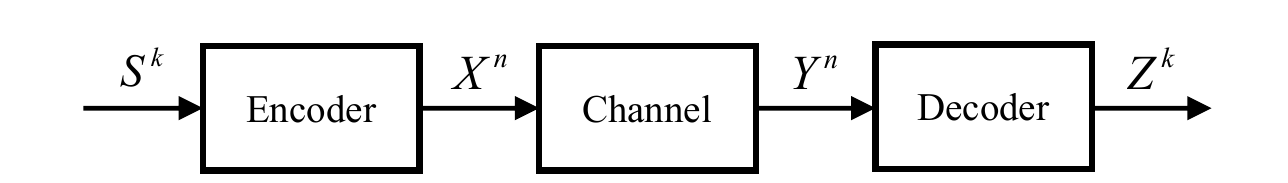
\includegraphics[width=0.85\linewidth]{fig/fig6.png}
\caption{결합 원천-채널 부호화의 시스템 모형.}
\end{figure}

\paragraph{1) 역 한계}
한편으로는 정보 확률변수를 바탕으로 일반적인 역 한계를 유도할 수 있다. 구체적으로, 상대 정보(relative information) $\iinf_{Y|X\|\bar{Y}}(x;y)=\log\frac{dP_{Y|X=x}}{dP_{\bar{Y}}}(y)$와 식~(8)의 $\dd$-기울인 정보 $\ttl_S(S,d)$의 차를 생각하면, 확률 $\P\bigl[\ttl_S(S,d)-\iinf_{Y|X\|\bar{Y}}(X;Y)\ge\gamma\bigr]$와 항 $e^{-\gamma}$의 차이가 초과 왜곡 확률 $\epsilon$을 넘지 않음을 보일 수 있다.\onote{원문 표현 그대로 옮겼다. [12]의 해당 정리를 식으로 쓰면 $\epsilon\ge\P\bigl[\ttl_S(S,d)-\iinf_{Y|X\|\bar{Y}}(X;Y)\ge\gamma\bigr]-e^{-\gamma}$ 꼴(임의의 $\gamma>0$과 $P_{\bar{Y}}$에 대해, 상황에 따라 $\sup$/$\inf$를 취함)로, 차이의 절댓값이 아니라 한쪽 방향 부등식이다.} 이 결과는 채널 입력의 형이 서로 다른 경우로 더 확장할 수도 있다.\onote{원문 ``extended when different channel input types''는 문장이 불완전하다. 채널 입력의 형별로 나누어 얻는 확장 한계를 가리키는 것으로 보고 옮겼다.} 다만 경우에 따라 이 방법으로 얻은 한계는 다소 느슨해진다.

다른 한편으로, Csiszár [55]는 $M$개 기호의 집합에서 원소 $L$개짜리 목록을 내놓는 목록 복호기를 써서 JSCC의 역 한계를 얻었다. Kostina 등 [12]은 이 기법을 유한 알파벳 원천에서 추상 알파벳 원천으로 확장하고, 여기에 가설 검정을 결합해 더 강한 역 한계를 얻었다.

\paragraph{2) 달성 가능성 한계}
최적 SSCC의 성능을 JSCC의 비점근 한계로 삼는 것은 자연스러운 발상이다. 실용적인 SSCC 방법 하나는 서로 독립인 무작위 원천 부호와 무작위 채널 부호를 쓰는 것이며, 이로부터 JSCC에 대해 계산 가능한 유한 부호 길이 달성 가능성 한계를 얻는다. 이 접근은 유한 부호 길이에서 SSCC가 왜 최적이 아닌지에 대해 중요한 통찰을 준다. 먼저 SSCC가 어떻게 점근적 한계에 도달하는지 보자. 부호 길이가 큰 영역에서 최적 원천 부호기의 출력은 대략 $\exp(kR(d))$개의 메시지로 이루어진 집합 위에서 거의 균등하게 분포하며, 이 메시지들이 정해진 왜곡 $d$ 이내에서 대부분의 원천 출력을 덮는다. 채널 부호화 정리에 따르면, 최대 우도(ML, maximum-likelihood) 복호기를 갖춘 채널 부호로 최대 $M=\exp(kR(d))<\exp(nC)$개의 메시지를 신뢰성 있게 구별할 수 있다. 따라서 최적의 원천 부호와 채널 부호를 이어 붙이면, $d>D(nC/k)$인 한 전체 방식의 초과 왜곡 확률은 무시할 만큼 작아진다. 그러나 유한 부호 길이에서는 최적 원천 부호기가 만드는 분포가 균등 분포와 거리가 멀다. 그 결과, 메시지 확률이 고르지 않다는 점을 고려하지 않고 ML 복호기를 쓰는 분리 방식은 최적에 가까운 비점근 성능에 이르지 못한다.

\paragraph{3) 근사}
JSCC 부호율의 가우스 근사를 소개하기 전에 몇 가지 조건을 밝혀 둔다. 원천과 채널은 정상이고 무기억이며, 왜곡 기준은 분리 가능하고 왜곡은 유계이다. 채널에 비용 함수가 있다면 그 비용 함수도 분리 가능해야 한다. 이 조건 아래에서 최적 $(k,n,d,\epsilon)$ 부호의 매개변수는 다음을 만족한다.
\begin{equation}
nC(\beta)-kR(d)=\sqrt{nV(\beta)+k\mathcal{V}(d)}\,Q^{-1}(\epsilon)+\theta(n),
\tag{34}
\end{equation}
여기서 $\mathcal{V}(d)$는 원천 분산도, $V(\beta)$는 채널 분산도이고, $\beta$는 채널 입력 비용 제약이다. 나머지 항 $\theta(n)$에 대해서는, 채널 입력 $X^n$과 출력 $Y^n$이 유한 알파벳 $\mathcal{X}$와 $\mathcal{Y}$ 위에서 정의되고 채널 비용 제약이 없으면 다음이 성립한다.
\begin{equation}
-c\log n+O(1)\le\theta(n)\le C_0\log n+\log\log n+O(1),
\tag{35}
\end{equation}
여기서 $c=|\mathcal{X}|-\frac{1}{2}$이고 $C_0=\frac{1}{2}+\frac{\Var\left(J'_{Z^\star}(\mathsf{S},\lambda^\star)\right)}{\E\left[|J''_{Z^\star}(\mathsf{S},\lambda^\star)|\right]\log e}$이며, $\lambda^\star=-\mathbb{R}'_{S}(d)$이다. 가우스 채널의 경우에 대한 추가 결과는 [12, Theorem 10]을 참고하라.

SSCC 아래의 근사는 [11]의 채널 부호화 결과와 [10]의 손실 원천 부호화 결과를 결합해 다음과 같이 얻는다.
\begin{equation}
nC(\beta)-kR(d)\le\min_{\eta+\zeta\le\epsilon}\left[\sqrt{nV(\beta)}\,Q^{-1}(\eta)+\sqrt{k\mathcal{V}(d)}\,Q^{-1}(\zeta)\right]+O(\log n).
\tag{36}
\end{equation}
채널과 원천 가운데 하나라도(또는 둘 다) 분산도가 0이면, 분리 부호화로도 결합 설계와 같은 전체 분산도를 달성할 수 있다. 이런 경우에는 $\dd$-기울인 정보나 채널 정보 밀도가 거의 결정적(deterministic)이어서, 최적 결합 원천-채널 부호가 이 확률적 양의 변동을 온전히 고려할 필요가 없기 때문이다.

\paragraph{4) SSCC와 JSCC의 비교}
식~(34)의 JSCC 근사와 식~(36)의 SSCC 근사를 비교하면, SSCC가 분리 설계 때문에 유한 부호 길이에서 성능을 잃는 이유를 더 직관적이고 간명하게 설명할 수 있다. 먼저 $k$와 $n$이 커질 때 CLT에 따라 $\dd$-기울인 정보와 채널 정보 밀도가 어떻게 행동하는지 보자. 원천이 정상이고 무기억이므로, 정규화한 $\dd$-기울인 정보 $J=\frac{1}{n}\ttl_{S^k}(S^k,d)$는 평균이 $\frac{k}{n}R(d)$이고 분산이 $\frac{k}{n}\frac{\mathcal{V}(d)}{n}$인 가우스 분포로 다가간다. 마찬가지로 조건부 정규화 채널 정보 밀도 $I=\frac{1}{n}\iinf^\star_{X^n;Y^n}(x^n;Y^{n\star})$는, 용량 달성 분포 아래에서 전형적인 모든 $x^n$에 대해 평균이 $C(\beta)$이고 분산이 $\frac{1}{n}V(\beta)$인 가우스 분포로 다가간다. 효율적인 부호기는 거의 모든 원천 실현값에 대해 이런 입력을 고르고, 원천과 채널은 서로 독립이다. 따라서 차 $I-J$ 역시 평균이 $C(\beta)-\frac{k}{n}R(d)$이고 분산이 $\frac{1}{n}\bigl(\frac{k}{n}\mathcal{V}(d)+V(\beta)\bigr)$인 가우스 분포에 가깝다.

JSCC에서는 식~(34)가 보여 주듯이, 채널 정보 밀도 $I$가 원천의 $\dd$-기울인 정보 $J$보다 클 때, 곧 사건 $\{I>J\}$가 일어날 때, 그리고 그때에만 원천을 왜곡 $d$ 이내로 복원할 수 있다. 반면 SSCC에서는 식~(36)이 보여 주듯이, 쌍 $(I,J)$가 두 반평면 $\{I>r\}$과 $\{J<r\}$의 교집합에 들어갈 때에만 높은 확률로 복원에 성공한다. 여기서 $r=\frac{\log M}{n}$은 원천 부호 블록과 채널 부호 블록 사이에 놓인 무잡음 채널의 용량을 나타낸다. 사건 $\{I>r\}\cap\{J<r\}$은 $\{I>J\}$의 진부분집합이므로, 분리 부호화 설계에서는 성능 손실이 생긴다.

\paragraph{5) JSCC의 최근 진전}
최근 연구는 실용적인 유한 부호 길이 통신 시스템에서 JSCC가 지닌 잠재력을 부각해 왔다. 과업 지향 JSCC 전략은 주어진 과업에 가장 관련 있는 정보만 전송하려 하며, 이는 저지연·대역폭 제약 환경에서 특히 유리하다 [60]. 딥러닝 기반 JSCC 방식은 유한 길이 원천 수열을 압축과 채널 부호화를 따로 거치지 않고 채널 입력으로 곧바로 사상할 수 있음을 보였다. 이런 방식은 채널 조건이 변해도 성능이 완만하게 저하되며, 짧은 부호 길이의 분리 기반 설계에서 흔히 나타나는 절벽 효과를 피한다 [61]. 더 나아가 JSCC에 채널 출력 되먹임을 도입하면 종단 간 복원 품질을 크게 높이고 전송 지연을 줄일 수 있다. 이는 유한 부호 길이 영역에서 현대 JSCC 기법이 지닌 구체적 이점을 보여 준다 [62].

\section{미해결 문제}

유한 부호 길이 정보이론에 많은 기여가 있었지만, 이 주제는 더 넓은 범위의 시나리오와 요구 조건에서 더 탐구되어야 한다. 이하에서는 이러한 미해결 문제와 향후 연구 방향 몇 가지를 자세히 논한다.

\subsection{촘촘하면서 해석적으로 다루기 쉬운 비점근 결과}

높은 정밀도와 해석적 다루기 쉬움을 함께 추구하는 일은 비점근 정보이론의 핵심 목표로 남아 있다. 기존 연구가 수많은 유한 부호 길이 한계와 근사를 유도했지만, 어떤 경우에는 엄밀한 정확도와 해석적 다루기 쉬움을 동시에 얻는 데 여전히 중대한 간극이 있다.

최근 [110]은 채널 부호화에서 중편차 영역의 3차 근사가 초단(超短) 부호 길이(예: $n=100$)와 극히 낮은 오류 확률(예: $10^{-10}$)에서도 놀라울 만큼 정확함을 보였다. 그러나 율-왜곡 문제에 대해서는 이에 상응하는 고차 근사가 아직 연구되지 않았으며, 이는 유망한 향후 연구 방향이다.

또한 대규모 무작위 접속에 필요한 최소 비트당 에너지에 대해, 수신 안테나가 하나인 페이딩 채널에서는 [49]가, MIMO 페이딩 채널에서는 [52, 53]이 비점근 달성 가능성 한계와 역 한계를 유도했다. 그러나 이 결과에는 복잡한 행렬 연산과 수치 최적화가 들어 있어 계산 부담이 크다. 따라서 해석적 촘촘함을 유지하면서도 복잡도가 낮은 비점근 한계가 필요하다. 아울러 계산 과정에 인공지능(AI, artificial intelligence) 기술 [127, 128]을 도입해 효율을 높이는 것도 흥미로운 방향이다.

\subsection{더 일반적인 시나리오의 비점근 결과}

단일 GMS의 경우, 율-왜곡 문제와 점진적 정밀화 문제의 2차 근사는 확립되었지만 다중 단말 손실 원천 부호화의 근본 한계는 여전히 미해결이다. 특히 GMS에 대한 Kaspi 문제의 비점근 달성 가능성 한계를 유도하는 일은 결코 간단하지 않다. 다중 기술(multiple descriptions) 문제에서는 GMS의 율-왜곡 영역이 확립되었지만 [129], 비점근 한계와 2차 근사를 유도하려면 새로운 기법이 필요하다.

채널 부호화에 관한 기존 비점근 결과도 더 일반적인 시나리오로 확장될 것으로 기대된다. 예를 들어 셀프리 대규모 MIMO는 넓어진 서비스 영역에서 많은 사용자를 지원하는 첨단 기법으로 제안되었다. 그러나 이러한 분산 안테나 시스템에서 채널 부호화의 유한 부호 길이 근본 한계는 아직 연구되지 않았다. 또한 기존 결과는 대부분 가우스 채널과 i.i.d.\ 페이딩 채널에 집중되어 있으며, 상관된 채널의 근본 한계는 여전히 미해결이다.

다중 원천, 페이딩 채널, 다중 수신 안테나처럼 더 넓은 부류의 원천과 채널에 대해 JSCC의 유한 부호 길이 근본 한계를 찾는 일은 매우 중요하며, 앞으로 다룰 만한 흥미로운 주제이다. 또한 의미 정보를 도입하는 것도 유망한 향후 연구 방향이다 [130, 131].

\subsection{효율적인 실용 방식 설계}

비점근 한계와 근사는 실용 통신 방식의 성능을 평가하는 이론적 기준점 역할을 한다. 기존 방식은 경우에 따라 이론적 결과와 상당한 격차를 보인다. 따라서 계산상 실현 가능성을 유지하면서 이론적 한계에 더 가까운 실용 방식을 개발하는 일이 꼭 필요하며, 이는 앞으로의 흥미로운 주제이다. 이 격차를 메우는 데 성공한다면, 새롭게 떠오르는 6G 사용 사례에서 지연에 민감한 응용을 지원하는 데 큰 의미가 있을 것이다.

\section{결론}

고전적인 점근 정보이론은 무한한 부호 길이와 페이로드 크기, 0으로 사라지는 오류 확률 같은 이상적인 가정에 기대고 있다. 그래서 지연에 민감한 실제 통신 시스템의 근본 한계를 규명하는 데에는 한계가 있다. 이런 이유로 저자들은 엄밀한 비점근 틀을 탐구하게 되었다. 이 작업에는 유한 부호 길이 영역의 난제를 풀 새로운 분석 도구와 기법이 필요하다. 이 논문에서는 비점근 근본 한계에 관한 최근 진전을 체계적으로 검토했다. 구체적으로, 정보이론적 비점근 근본 한계에 대한 다양한 비점근 달성 가능성 한계, 역 한계, 근사를 각 결과의 바탕에 있는 핵심 아이디어와 함께 제시했다. 먼저 원천 부호화의 기초 결과에서 출발해, P2P와 다중 단말 경우의 무손실 압축과 손실 압축을 모두 엄밀하게 분석했다. 이 과정에서 무기억 원천 모형과 기억이 있는 원천 모형을 아우르고, 원천 분포를 완전히 아는 경우와 통계적으로 불일치하는 경우를 모두 다루었다. 채널 부호화에 대해서는 P2P 시스템에서 데이터율, 오류 확률, 부호 길이 사이의 상충 관계에 관한 유한 부호 길이 결과를 논하고, 이어서 다중 접속 채널과 새로 떠오르는 대규모 접속 채널의 최근 진전을 다루었다. 나아가 JSCC의 비점근 결과를 제시했다. JSCC는 유한 부호 길이에서 분리 방식보다 상당한 성능 이점을 주는 것으로 나타났는데, 이는 고전적인 점근 정보이론의 결론과 다르다. 점근 지표에서 유한 부호 길이 정보이론으로 옮겨 가는 패러다임 전환 덕분에, 실제로 의미 있는 시나리오의 성능을 정확하게 규명할 수 있다. 또한 비점근 영역에서 근본 한계가 어떻게 행동하는지 알면 실용 방식을 평가할 수 있다. 실제로 실용 방식은 경우에 따라 이론적 결과와 큰 격차를 보였다. 끝으로 유한 부호 길이 정보이론의 미해결 과제 몇 가지를 논했다. 이 과제들은 미래 무선 통신 시스템을 위한 정보이론적 분석을 발전시키는 데 꼭 필요하다.


\clearpage
\renewcommand{\refname}{참고문헌}
\begin{thebibliography}{131}\small
\bibitem{r1} ITU-R, M.2160: Framework and overall objectives of the future development of IMT for 2030 and beyond, \url{https://www.itu.int/rec/R-REC-M.2160/en}, [Online] (2023).
\bibitem{r2} 3GPP, Service requirements for the 5G system, TS 22.261 V19.5.0., Release 19 (2023).
\bibitem{r3} 3GPP, Study on physical layer enhancements for NR ultra-reliable and low latency case (URLLC), TR 38.824 V16.0.0., Release 16 (2019).
\bibitem{r4} X. You, Y. Huang, S. Liu, D. Wang, J. Ma, C. Zhang, H. Zhan, C. Zhang, J. Zhang, Z. Liu, et al., Toward 6G TK$\mu$ extreme connectivity: Architecture, key technologies and experiments, IEEE Wireless Commun. 30 (3) (2023) 86--95.
\bibitem{r5} A. Pourkabirian, M. S. Kordafshari, A. Jindal, M. H. Anisi, A vision of 6G URLLC: Physical-layer technologies and enablers, IEEE Commun. Standards Mag. 8 (2) (2024) 20--27.
\bibitem{r6} Y. Huang, Challenges and opportunities of sub-6 GHz integrated sensing and communications for 5G-advanced and beyond, Chinese J. Electron. 33 (2) (2024) 323--325.
\bibitem{r7} Y. Li, J. Zhao, J. Liao, F. Hu, Cellular v2x-based integrated sensing and communication system: Feasibility and performance analysis, Chinese J. Electron. 33 (4) (2024) 1104--1116.
\bibitem{r8} C. E. Shannon, A mathematical theory of communication, Bell Syst. Tech. J. 27 (3) (1948) 379--423.
\bibitem{r9} I. Kontoyiannis, S. Verdú, Optimal lossless data compression: Non-asymptotics and asymptotics, IEEE Trans. Inform. Theory 60 (2) (2013) 777--795.
\bibitem{r10} V. Kostina, S. Verdú, Fixed-length lossy compression in the finite blocklength regime, IEEE Trans. Inform. Theory 58 (6) (2012) 3309--3338.
\bibitem{r11} Y. Polyanskiy, H. V. Poor, S. Verdú, Channel coding rate in the finite blocklength regime, IEEE Trans. Inform. Theory 56 (5) (2010) 2307--2359.
\bibitem{r12} V. Kostina, S. Verdú, Lossy joint source-channel coding in the finite blocklength regime, IEEE Trans. Inform. Theory 59 (5) (2013) 2545--2575.
\bibitem{r13} L. Zhou, M. Motani, et al., Finite blocklength lossy source coding for discrete memoryless sources, Foundations and Trends\textregistered{} in Communications and Information Theory 20 (3) (2023) 157--389.
\bibitem{r14} V. Kostina, Lossy data compression: nonasymptotic fundamental limits, Ph.D.\ thesis, Princeton University (2013).
\bibitem{r15} S. Verdú, Teaching it, in: Proc. IEEE Int. Symp. Inf. Theory (ISIT), IEEE, 2007, pp. ix--ix.
\bibitem{r16} I. Kontoyiannis, Pointwise redundancy in lossy data compression and universal lossy data compression, IEEE Trans. Inform. Theory 46 (1) (2000) 136--152.
\bibitem{r17} K. Marton, Error exponent for source coding with a fidelity criterion, IEEE Trans. Inform. Theory 20 (2) (1974) 197--199.
\bibitem{r18} T. S. Han, The reliability functions of the general source with fixed-length coding, IEEE Trans. Inform. Theory 46 (6) (2006) 2117--2132.
\bibitem{r19} K. Iriyama, Probability of error for the fixed-length source coding of general sources, IEEE Trans. Inform. Theory 47 (4) (2001) 1537--1543.
\bibitem{r20} E.-h. Yang, Z. Zhang, On the redundancy of lossy source coding with abstract alphabets, IEEE Trans. Inform. Theory 45 (4) (1999) 1092--1110.
\bibitem{r21} R. Gray, Information rates of autoregressive processes, IEEE Trans. Inform. Theory 16 (4) (1970) 412--421.
\bibitem{r22} P. Tian, V. Kostina, The dispersion of the Gauss--Markov source, IEEE Trans. Inform. Theory 65 (10) (2019) 6355--6384.
\bibitem{r23} P. Tian, V. Kostina, Nonstationary Gauss-Markov processes: Parameter estimation and dispersion, IEEE Trans. Inform. Theory 67 (4) (2021) 2426--2449.
\bibitem{r24} A. Lapidoth, On the role of mismatch in rate distortion theory, IEEE Trans. Inform. Theory 43 (1) (1997) 38--47.
\bibitem{r25} L. Zhou, V. Y. Tan, M. Motani, Refined asymptotics for rate-distortion using Gaussian codebooks for arbitrary sources, IEEE Trans. Inform. Theory 65 (5) (2018) 3145--3159.
\bibitem{r26} A. H. Kaspi, Rate-distortion function when side-information may be present at the decoder, IEEE Trans. Inform. Theory 40 (6) (2002) 2031--2034.
\bibitem{r27} L. Zhou, M. Motani, Non-asymptotic converse bounds and refined asymptotics for two source coding problems, IEEE Trans. Inform. Theory 65 (10) (2019) 6414--6440.
\bibitem{r28} A. No, A. Ingber, T. Weissman, Strong successive refinability and rate-distortion-complexity tradeoff, IEEE Trans. Inform. Theory 62 (6) (2016) 3618--3635.
\bibitem{r29} L. Zhou, V. Y. Tan, M. Motani, Second-order and moderate deviations asymptotics for successive refinement, IEEE Trans. Inform. Theory 63 (5) (2017) 2896--2921.
\bibitem{r30} B. Rimoldi, Successive refinement of information: Characterization of the achievable rates, IEEE Trans. Inform. Theory 40 (1) (1994) 253--259.
\bibitem{r31} M. Effros, Distortion-rate bounds for fixed-and variable-rate multiresolution source codes, IEEE Trans. Inform. Theory 45 (6) (1999) 1887--1910.
\bibitem{r32} W. Yang, A. Collins, G. Durisi, Y. Polyanskiy, H. V. Poor, Beta--beta bounds: Finite-blocklength analog of the golden formula, IEEE Trans. Inform. Theory 64 (9) (2018) 6236--6256.
\bibitem{r33} Y. Polyanskiy, H. V. Poor, S. Verdu, Feedback in the non-asymptotic regime, IEEE Trans. Inform. Theory 57 (8) (2011) 4903--4925.
\bibitem{r34} R. C. Yavas, V. Y. Tan, Variable-length feedback codes over known and unknown channels with non-vanishing error probabilities, IEEE Trans. Inform. Theory 71 (5) (2025) 3271--3286.
\bibitem{r35} Y. Polyanskiy, S. Verdú, Arimoto channel coding converse and Rényi divergence, in: Proc. 48th Allerton Conf. Commun., IEEE, 2010, pp. 1327--1333.
\bibitem{r36} W. Yang, G. Durisi, T. Koch, Y. Polyanskiy, Quasi-static multiple-antenna fading channels at finite blocklength, IEEE Trans. Inform. Theory 60 (7) (2014) 4232--4265.
\bibitem{r37} Y. Polyanskiy, S. Verdú, Scalar coherent fading channel: Dispersion analysis, in: Proc. IEEE Int. Symp. Inf. Theory (ISIT), IEEE, 2011, pp. 2959--2963.
\bibitem{r38} A. Collins, Y. Polyanskiy, Coherent multiple-antenna block-fading channels at finite blocklength, IEEE Trans. Inform. Theory 65 (1) (2019) 380--405.
\bibitem{r39} J. Hoydis, R. Couillet, P. Piantanida, The second-order coding rate of the MIMO quasi-static Rayleigh fading channel, IEEE Trans. Inform. Theory 61 (12) (2015) 6591--6622.
\bibitem{r40} X. You, B. Sheng, Y. Huang, W. Xu, C. Zhang, D. Wang, P. Zhu, C. Ji, Closed-form approximation for performance bound of finite blocklength massive MIMO transmission, IEEE Trans. Commun. 71 (12) (2023) 6939--6951.
\bibitem{r41} Y. Polyanskiy, S. Verdú, Channel dispersion and moderate deviations limits for memoryless channels, in: Proc. Allerton Conf. Commun., Contr., Comput., IEEE, 2010, pp. 1334--1339.
\bibitem{r42} Y. Altuǧ, A. B. Wagner, Moderate deviations in channel coding, IEEE Trans. Inform. Theory 60 (8) (2014) 4417--4426.
\bibitem{r43} E. MolavianJazi, J. N. Laneman, A second-order achievable rate region for Gaussian multi-access channels via a central limit theorem for functions, IEEE Trans. Inform. Theory 61 (12) (2015) 6719--6733.
\bibitem{r44} Y.-W. Huang, P. Moulin, Finite blocklength coding for multiple access channels, in: Proc. IEEE Int. Symp. Inf. Theory (ISIT), IEEE, 2012, pp. 831--835.
\bibitem{r45} E. Haim, Y. Kochman, U. Erez, A note on the dispersion of network problems, in: Proc. IEEE Conv. Elect. Electron. Eng. Israel (IEEEI), IEEE, 2012, pp. 1--9.
\bibitem{r46} J. Scarlett, A. Martinez, A. G. i Fàbregas, Second-order rate region of constant-composition codes for the multiple-access channel, IEEE Trans. Inform. Theory 61 (1) (2015) 157--172.
\bibitem{r47} J. Scarlett, V. Y. Tan, Second-order asymptotics for the gaussian mac with degraded message sets, IEEE Trans. Inform. Theory 61 (12) (2015) 6700--6718.
\bibitem{r48} Y. Polyanskiy, A perspective on massive random-access, in: Proc. IEEE Int. Symp. Inf. Theory (ISIT), IEEE, 2017, pp. 2523--2527.
\bibitem{r49} S. S. Kowshik, K. Andreev, A. Frolov, Y. Polyanskiy, Energy efficient coded random access for the wireless uplink, IEEE Trans. Commun. 68 (8) (2020) 4694--4708.
\bibitem{r50} Y. Han, Z. Xiong, A. Høst-Madsen, Finite blocklength analysis of energy-delay tradeoff in uncoordinated mac, IEEE Trans. Commun. (2025).
\bibitem{r51} K.-H. Ngo, A. Lancho, G. Durisi, A. G. i Amat, Unsourced multiple access with random user activity, IEEE Trans. Inform. Theory 69 (7) (2023) 4537--4558.
\bibitem{r52} J. Gao, Y. Wu, S. Shao, W. Yang, H. V. Poor, Energy efficiency of massive random access in MIMO quasi-static Rayleigh fading channels with finite blocklength, IEEE Trans. Inform. Theory 69 (3) (2023) 1618--1657.
\bibitem{r53} J. Gao, Y. Wu, T. Li, W. Zhang, Energy efficiency of MIMO massive unsourced random access with finite blocklength, IEEE Wireless Commun. Lett. 12 (4) (2023) 743--747.
\bibitem{r54} J. Gao, Y. Wu, G. Caire, W. Yang, H. V. Poor, W. Zhang, Unsourced random access in MIMO quasi-static Rayleigh fading channels: Finite blocklength and scaling law analyses, IEEE Trans. Inform. Theory, early access (2025).
\bibitem{r55} I. Csiszár, On the error exponent of source-channel transmission with a distortion threshold, IEEE Trans. Inform. Theory 28 (6) (1982) 823--828.
\bibitem{r56} R. Pilc, The transmission distortion of a source as a function of the encoding block length, Bell Syst. Tech. J. 47 (6) (1968) 827--885.
\bibitem{r57} A. D. Wyner, On the transmission of correlated Gaussian data over a noisy channel with finite encoding block length, Inf. Contr. 20 (3) (1972) 193--215.
\bibitem{r58} I. Csiszár, J. Korner, Graph decomposition: A new key to coding theorems, IEEE Trans. Inform. Theory 27 (1) (1981) 5--12.
\bibitem{r59} D. Wang, A. Ingber, Y. Kochman, The dispersion of joint source-channel coding, in: Proc. Allerton Conf. Commun., Control, Comput., IEEE, 2011, pp. 180--187.
\bibitem{r60} D. Gündüz, M. A. Wigger, T.-Y. Tung, P. Zhang, Y. Xiao, Joint source--channel coding: Fundamentals and recent progress in practical designs, Proceedings of the IEEE (2024).
\bibitem{r61} E. Bourtsoulatze, D. B. Kurka, D. Gündüz, Deep joint source-channel coding for wireless image transmission, IEEE Tran. Cogn. Netw. 5 (3) (2019) 567--579.
\bibitem{r62} D. B. Kurka, D. Gündüz, DeepJSCC-f: Deep joint source-channel coding of images with feedback, IEEE J. Sel. Areas Inf. Theory 1 (1) (2020) 178--193.
\bibitem{r63} G. Wade, Signal coding and processing, Cambridge university press, 1994.
\bibitem{r64} S. Verdú, Teaching lossless data compression, IEEE Inform. Theory Society Newsletter 61 (1) (2011) 18--19.
\bibitem{r65} Y. Polyanskiy, Channel coding: Non-asymptotic fundamental limits, Ph.D.\ thesis, Princeton University, Princeton, NJ, USA (2010).
\bibitem{r66} T. M. Cover, J. A. Thomas, Elements of information theory, 2nd ed. New Jersey: Wiley, 2006.
\bibitem{r67} I. Kontoyiannis, Second-order noiseless source coding theorems, IEEE Trans. Inform. Theory 43 (4) (1997) 1339--1341.
\bibitem{r68} N. Merhav, Universal coding with minimum probability of codeword length overflow, IEEE Trans. Inform. Theory 37 (3) (1991) 556--563.
\bibitem{r69} T. A. Welch, A technique for high-performance data compression, Computer 17 (06) (1984) 8--19.
\bibitem{r70} I. Csiszár, J. Körner, Information theory: coding theorems for discrete memoryless systems, Cambridge University Press, 2011.
\bibitem{r71} W. Szpankowski, S. Verdú, Minimum expected length of fixed-to-variable lossless compression without prefix constraints, IEEE Trans. Inform. Theory 57 (7) (2011) 4017--4025.
\bibitem{r72} A. A. Yushkevich, On limit theorems connected with the concept of entropy of Markov chains, Uspekhi Matematicheskikh Nauk 8 (5) (1953) 177--180.
\bibitem{r73} V. Strassen, Asymptotische abschätzugen in Shannon’s informationstheorie, in: Proc. Trans. 3rd Prague Conf. Inf. Theory, 1962, pp. 689--723.
\bibitem{r74} V. V. Petrov, Limit Theorems of Probability Theory: Sequences of Independent Random Variables, Oxford, U.K.: Oxford Science, 1995.
\bibitem{r75} C. E. Shannon, et al., Coding theorems for a discrete source with a fidelity criterion, IRE Nat. Conv. Rec 4 (142-163) (1959) 1.
\bibitem{r76} J. Körner, et al., Coding of an information source having ambiguous alphabet and the entropy of graphs, in: 6th Prague conference on Information Theory, Academia, Prague, 1971, pp. 411--425.
\bibitem{r77} J. C. Kieffer, Strong converses in source coding relative to a fidelity criterion, IEEE Trans. Inform. Theory 37 (2) (1991) 257--262.
\bibitem{r78} S. Verdú, ELE528: Information theory lecture notes, Princeton University (2009).
\bibitem{r79} T. J. Goblick, Coding for a discrete information source with a distortion measure, Ph.D.\ thesis, Massachusetts Institute of Technology (1963).
\bibitem{r80} J. T. Pinkston, Encoding independent sample information sources. (1967).
\bibitem{r81} D. Sakrison, A geometric treatment of the source encoding of a Gaussian random variable, IEEE Trans. Inform. Theory 14 (3) (1968) 481--486.
\bibitem{r82} D. Varodayan, A. Aaron, B. Girod, Exploiting spatial correlation in pixel-domain distributed image compression, in: Proc. Picture Coding Symposium, Beijing, China, 2006.
\bibitem{r83} N. D. Memon, K. Sayood, Lossless compression of video sequences, IEEE Trans. Commun. 44 (10) (1996) 1340--1345.
\bibitem{r84} A. Kolmogorov, On the shannon theory of information transmission in the case of continuous signals, IRE Transactions on Information Theory 2 (4) (1956) 102--108.
\bibitem{r85} T. Berger, Information rates of Wiener processes, IEEE Trans. Inform. Theory 16 (2) (1970) 134--139.
\bibitem{r86} L. D. Davisson, Rate-distortion theory and application, Proceedings of the IEEE 60 (7) (1972) 800--808.
\bibitem{r87} I. Dumer, M. S. Pinsker, V. V. Prelov, On coverings of ellipsoids in Euclidean spaces, IEEE Trans. Inform. Theory 50 (10) (2004) 2348--2356.
\bibitem{r88} W. H. Equitz, T. M. Cover, Successive refinement of information, IEEE Trans. Inform. Theory 37 (2) (1991) 269--275.
\bibitem{r89} V. Kostina, S. Verdú, A new converse in rate-distortion theory, in: 2012 46th Annual Conference on Information Sciences and Systems (CISS), IEEE, 2012, pp. 1--6.
\bibitem{r90} S.-Q. Le, V. Y. Tan, M. Motani, Second-order coding rates for conditional rate-distortion, arXiv preprint arXiv:1410.2687 (2014).
\bibitem{r91} A. Kanlis, P. Narayan, Error exponents for successive refinement by partitioning, IEEE Trans. Inform. Theory 42 (1) (1996) 275--282.
\bibitem{r92} E. Tuncel, K. Rose, Error exponents in scalable source coding, IEEE Trans. Inform. Theory 49 (1) (2003) 289--296.
\bibitem{r93} V. Y. Tan, O. Kosut, On the dispersions of three network information theory problems, IEEE Trans. Inform. Theory 60 (2) (2013) 881--903.
\bibitem{r94} A. Feinstein, A new basic theorem of information theory, IRE Trans. Inform. Theory 4 (4) (1954) 2--22.
\bibitem{r95} C. E. Shannon, Certain results in the coding theory for noisy channels, Inf. Contr. 1 (1957) 6--25.
\bibitem{r96} R. G. Gallager, A simple derivation of the coding theorem and some applications, IEEE Trans. Inform. Theory 11 (1) (1965) 3--18.
\bibitem{r97} J. Scarlett, Reliable communication under mismatched decoding, Ph.D.\ thesis, University of Cambridge, Trinity Hall, Cambridge, UK (2014).
\bibitem{r98} W. Yang, R. F. Schaefer, H. V. Poor, Wiretap channels: Nonasymptotic fundamental limits, IEEE Trans. Inform. Theory 65 (7) (2019) 4069--4093.
\bibitem{r99} C. E. Shannon, Probability of error for optimal codes in a Gaussian channel, Bell Syst. Tech. J. 38 (3) (1959) 611--656.
\bibitem{r100} R. G. Gallager, Information theory and reliable communication, Wiley, New York, 1968.
\bibitem{r101} J. Wolfowitz, The coding of messages subject to chance errors, Illinois J. Math. 1 (1957) 591--606.
\bibitem{r102} C. E. Shannon, R. G. Gallager, E. R. Berlekamp, Lower bounds to error probability for coding on discrete memoryless channels I, Inf. Contr. 10 (1967) 65--103.
\bibitem{r103} S. Verdú, T. S. Han, A general formula for channel capacity, IEEE Trans. Inform. Theory 40 (4) (1994) 1147--1157.
\bibitem{r104} L. Shen, Y. Wu, Y. Xu, X. You, X. Gao, W. Zhang, GLDPC-PC codes: Channel coding towards 6G communications, accepted by IEEE Commun. Mag., arXiv preprint arXiv:2404.14828 (2025).
\bibitem{r105} P. Yuan, K. R. Duffy, M. Médard, Soft-output successive cancellation list decoding, IEEE Trans. Inform. Theory 71 (2) (2025) 1007--1017.
\bibitem{r106} L. Shen, Y. Wu, Y. Xu, X. You, X. Gao, W. Zhang, Soft-output fast successive-cancellation list decoder for polar codes, in: Proc. IEEE Wireless Commun. Netw. Conf. (WCNC), IEEE, 2025, pp. 1--6.
\bibitem{r107} W. Yang, G. Durisi, T. Koch, Y. Polyanskiy, Diversity versus channel knowledge at finite block-length, in: Proc. IEEE Inf. Theory Workshop (ITW), IEEE, 2012, pp. 572--576.
\bibitem{r108} F. Ye, X. You, J. Li, C. Zhang, C. Ji, Explicit performance bound of finite blocklength coded MIMO: Time-domain versus spatiotemporal channel coding, arXiv preprint arXiv:2406.13922v2 (2024).
\bibitem{r109} X. You, 6G extreme connectivity via exploring spatiotemporal exchangeability, Sci. China Inf. Sci. 66 (3) (2023) 130306.
\bibitem{r110} R. C. Yavas, V. Kostina, M. Effros, Third-order analysis of channel coding in the small-to-moderate deviations regime, IEEE Trans. Inform. Theory (2024).
\bibitem{r111} A. D. Wyner, Recent results in the shannon theory, IEEE Trans. Inform. Theory 20 (1) (1974) 2--10.
\bibitem{r112} Y. Wu, X. Gao, S. Zhou, W. Yang, Y. Polyanskiy, G. Caire, Massive access for future wireless communication systems, IEEE Wireless Commun. 27 (4) (2020) 148--156.
\bibitem{r113} L. Liu, W. Yu, Massive connectivity with massive MIMO---Part I: Device activity detection and channel estimation, IEEE Trans. Signal Process. 66 (11) (2018) 2933--2946.
\bibitem{r114} L. Liu, E. G. Larsson, W. Yu, P. Popovski, C. Stefanovic, E. De Carvalho, Sparse signal processing for grant-free massive connectivity: A future paradigm for random access protocols in the Internet of Things, IEEE Signal Process. Mag. 35 (5) (2018) 88--99.
\bibitem{r115} X. Chen, T.-Y. Chen, D. Guo, Capacity of Gaussian many-access channels, IEEE Trans. Inform. Theory 63 (6) (2017) 3516--3539.
\bibitem{r116} I. Zadik, Y. Polyanskiy, C. Thrampoulidis, Improved bounds on Gaussian mac and sparse regression via Gaussian inequalities, in: Proc. IEEE Int. Symp. Inf. Theory (ISIT), IEEE, 2019, pp. 430--434.
\bibitem{r117} S. S. Kowshik, Y. Polyanskiy, Fundamental limits of many-user mac with finite payloads and fading, IEEE Trans. Inform. Theory 67 (9) (2021) 5853--5884.
\bibitem{r118} J. Gao, Y. Wu, W. Zhang, Energy-efficiency of massive random access with individual codebook, in: Proc. IEEE Global Commun. (GLOBECOM), IEEE, 2020, pp. 1--6.
\bibitem{r119} A. Fengler, S. Haghighatshoar, P. Jung, G. Caire, Non-bayesian activity detection, large-scale fading coefficient estimation, and unsourced random access with a massive MIMO receiver, IEEE Trans. Inform. Theory 67 (5) (2021) 2925--2951.
\bibitem{r120} M. J. Ahmadi, M. Kazemi, T. M. Duman, Unsourced random access using multiple stages of orthogonal pilots: MIMO and single-antenna structures, IEEE Trans. Wireless Commun. 23 (2) (2024) 1343--1355.
\bibitem{r121} A. Fengler, O. Musa, P. Jung, G. Caire, Pilot-based unsourced random access with a massive MIMO receiver, interference cancellation, and power control, IEEE J. Sel. Areas Commun. 40 (5) (2022) 1522--1534.
\bibitem{r122} M. Gkagkos, K. R. Narayanan, J.-F. Chamberland, C. N. Georghiades, Fasura: A scheme for quasi-static fading unsourced random access channels, IEEE Trans. Commun. 71 (11) (2023) 6391--6401.
\bibitem{r123} A. Decurninge, I. Land, M. Guillaud, Tensor-based modulation for unsourced massive random access, IEEE Wireless Commun. Lett. 10 (3) (2021) 552--556.
\bibitem{r124} R. J. Pilc, Coding theorems for discrete source-channel pairs, Ph.D.\ thesis, Massachusetts Institute of Technology (1967).
\bibitem{r125} A. Wyner, Communication of analog data from a Gaussian source over a noisy channel, Bell Syst. Tech. J. 47 (5) (1968) 801--812.
\bibitem{r126} A. T. Campo, G. Vazquez-Vilar, A. G. i Fabregas, A. Martinez, Random-coding joint source-channel bounds, in: Proc. IEEE Int. Symp. Inf. Theory (ISIT), IEEE, 2011, pp. 899--902.
\bibitem{r127} X. Wang, C. Li, Z. Sun, L. Hui, Review of GAN-based research on Chinese character font generation, Chinese J. Electron. 33 (3) (2024) 584--600.
\bibitem{r128} S. Yue, Y. Deng, G. Wang, J. Ren, Y. Zhang, Federated offline reinforcement learning with proximal policy evaluation, Chinese J. Electron. 33 (6) (2024) 1360--1372.
\bibitem{r129} L. Ozarow, On a source-coding problem with two channels and three receivers, Bell Syst. Tech. J. 59 (10) (1980) 1909--1921.
\bibitem{r130} P. Zhang, G. Shi, S. Cui, Z. Zhang, K. Niu, Y. Xiao, Z. Qin, J. Dai, S. Shao, G. Deniz, G. Eleonora, Semantic communications: Theories, technologies and applications, China Commun. 21 (7) (2024) iii--vii.
\bibitem{r131} H. Tang, H. Zhu, H. Wei, H. Zheng, X. Mao, M. Lu, J. Guo, Representation of semantic word embeddings based on SLDA and Word2vec model, Chinese J. Electron. 32 (3) (2023) 647--654.
\end{thebibliography}


\end{document}
